\section{Empirical Results}
\label{sec:results}

Unless a table or figure note states otherwise, estimates are displayed to four decimal places, correlations to three decimal places, and counts as integers. Monte Carlo $p$-values are reported at the resolution supported by the number of simulations, including the minimum attainable value where relevant.

The empirical results follow the sequence defined by the integrated framework presented in Section~\ref{sec:methodology}. We begin by examining the statistical behavior of individual returns and the dependence structure across B3 equities. We then investigate whether this dependence contains components that extend beyond broad market synchronization and sampling noise. 

The resulting spectral structures are subsequently examined through hierarchical and network representations to determine how market-mode removal changes the organization of asset dependencies. Finally, we assess the robustness and temporal behavior of these structural findings before testing whether the descriptors improve realized-volatility forecast accuracy.

Each stage therefore builds on the evidence obtained in the previous one. The correlation analysis establishes the empirical dependency structure; RMT separates broad collective behavior from smaller structural components; clustering and financial networks reveal how these components are organized across assets; and the final retrospective model assessment tests whether adding these descriptors improves volatility forecast accuracy.

\subsection{Stylized Facts: From Return Dynamics to Market Dependence}
\label{sec:stylized_correlation}

Building on the concepts introduced in Section~\ref{subsec:theory_market_dynamics}, we begin by examining whether the B3 data exhibit the empirical properties commonly observed in financial returns. We first consider the three representative assets defined in Section~\ref{subsec:stylized_method} and then extend the analysis from individual return dynamics to the cross-sectional dependence structure of the broader equity universe. This progression establishes the empirical basis for the spectral decomposition and network analyses that follow.

The selected assets show several familiar return properties: price trajectories differ over the long run, large daily moves cluster in time, and absolute returns remain autocorrelated. Figure~\ref{fig:stylized_facts} brings these complementary diagnostics together for PETR4, VALE3 and BBDC4: normalized prices, daily returns, the complementary cumulative distribution of absolute returns and their autocorrelation \cite{cont_2001_empirical}.

The normalized-price trajectories differ substantially across the three assets, reflecting their distinct long-run dynamics. Their daily returns nevertheless share several common empirical features. Large movements tend to occur in temporally concentrated periods, indicating volatility clustering, while the complementary cumulative distributions show that large absolute returns occur more frequently than expected under a Gaussian benchmark. The autocorrelation of absolute returns remains positive over several lags, providing further evidence of persistent volatility \cite{cont_2001_empirical}.

Table~\ref{tab:descriptive_stats} quantifies the same diagnostics. All three series have means close to zero, substantial kurtosis and non-negligible counts of large absolute returns. PETR4 has the largest negative daily observation in the 2006--2025 window, while VALE3 and BBDC4 also show stress-period extremes. The autocorrelations of absolute returns remain positive across several lags, especially for VALE3.

\begin{center}
\captionof{table}{Descriptive statistics for the three demonstration assets, 2006--2025.}
\label{tab:descriptive_stats}
\scriptsize
\setlength{\tabcolsep}{2.8pt}
\resizebox{\linewidth}{!}{%
\begin{tabular}{lrrrrrrrrrrrrrrr}
\toprule
Symbol & $n$ & Mean & Std. & Skew. & Ex. kurt. & Min. & Max. &
VaR$_{1\%}$ & VaR$_{5\%}$ &
$|r|>10\%$ & $|r|>20\%$ &
ACF$_1$ & ACF$_5$ & ACF$_{20}$ & ACF$_{60}$ \\
\midrule
BBDC4 & 4953 & 0.0003 & 0.0218 &  0.02 &  7.96 & -0.1910 & 0.1999 & -0.0559 & -0.0312 & 16 & 0 & 0.207 & 0.174 & 0.122 & 0.044 \\
PETR4 & 4953 & 0.0004 & 0.0276 & -0.76 & 11.55 & -0.3524 & 0.2007 & -0.0767 & -0.0408 & 41 & 4 & 0.254 & 0.209 & 0.140 & 0.062 \\
VALE3 & 4953 & 0.0005 & 0.0258 & -0.22 &  7.51 & -0.2814 & 0.1936 & -0.0676 & -0.0381 & 26 & 2 & 0.231 & 0.207 & 0.169 & 0.119 \\
\bottomrule
\end{tabular}}
\end{center}

\noindent\footnotesize\emph{Notes:} Mean, Std., extrema and VaR are reported to four decimal places; skewness and excess kurtosis to two; autocorrelations to three; and event counts as integers. Mean and Std. are computed from daily log returns. VaR$_{1\%}$ and VaR$_{5\%}$ are empirical lower-tail return quantiles, and ACF$_\ell$ is the autocorrelation of absolute returns at lag $\ell$ trading days.

\begin{center}
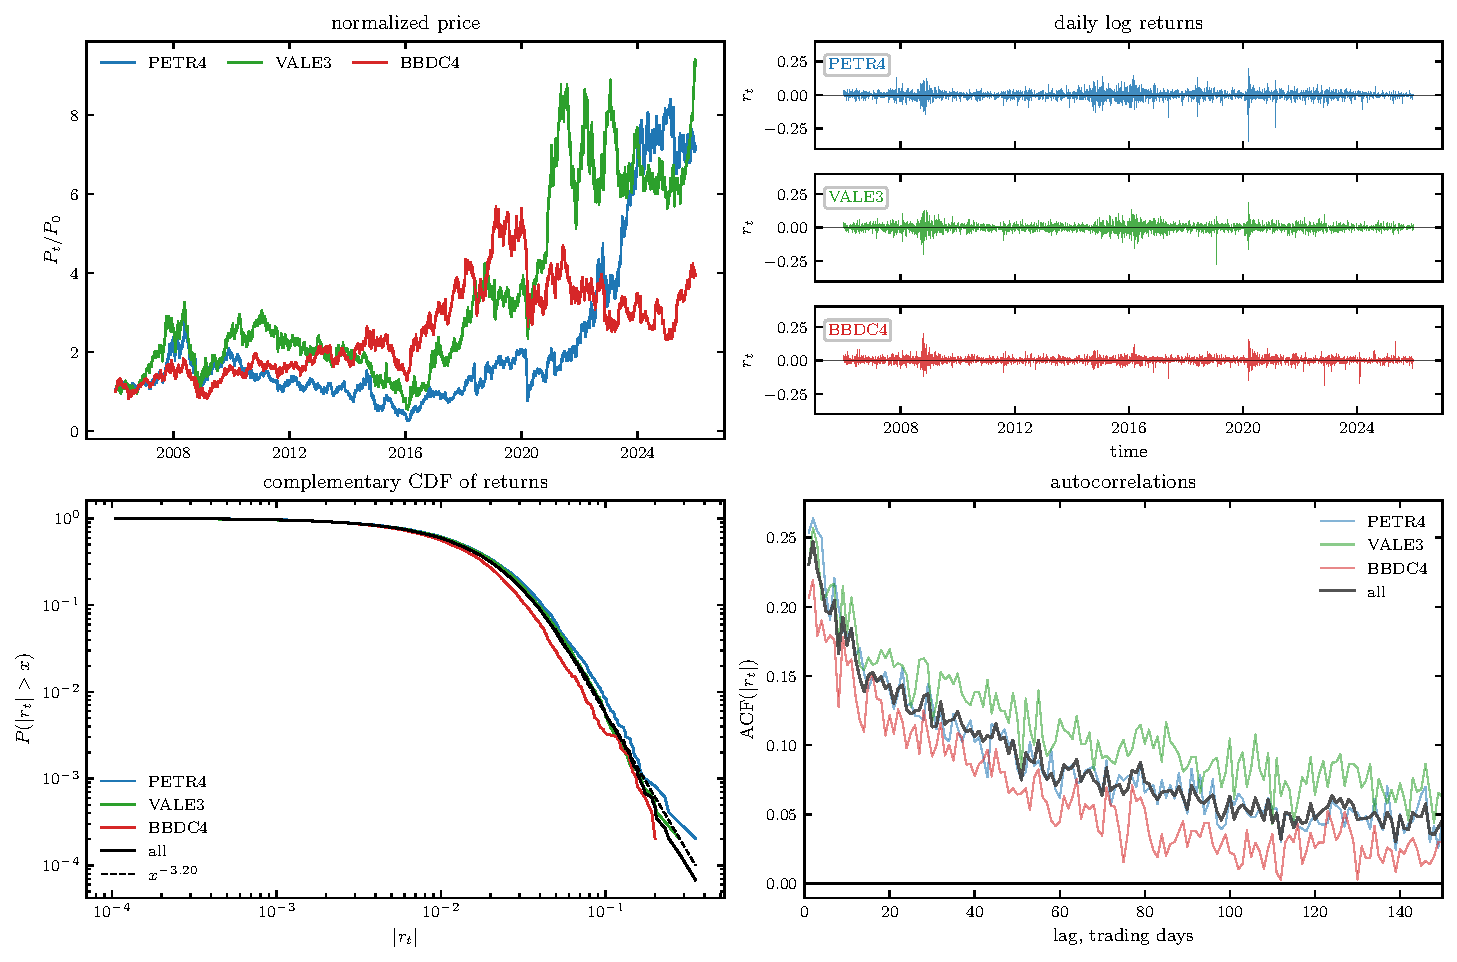
\includegraphics[width=0.95\linewidth]{images/figure_1d_stylized_facts_demo_assets_clean_2006_2025.pdf}
\captionof{figure}{Stylized facts for PETR4, VALE3 and BBDC4 over 2006--2025. The panels show normalized prices, daily log returns, the complementary cumulative distribution of absolute returns and autocorrelations of absolute returns. The return panel uses three vertically aligned subpanels with a common scale and a zero reference line for each asset.}
\label{fig:stylized_facts}
\end{center}

\normalsize

Taken together, the visual and numerical evidence shows that the selected B3 assets exhibit well-known empirical regularities of financial returns, including non-Gaussian behavior and volatility persistence. This motivates extending the analysis from individual return dynamics to the dependence structure across the broader equity universe.

We now turn from individual return behaviour to cross-sectional dependence. The core historical universe contains 58 assets, producing $N(N-1)/2=1653$ unique asset pairs. The static summaries use the available overlap for each pair and therefore retain the broader unbalanced historical coverage. The subsequent RMT analysis instead uses the complete synchronized 58-asset panel from 23 August 2006 to 15 August 2024. This distinction ensures that the descriptive correlation evidence is not confused with the common-sample correlation matrix used for the spectral decomposition. 

The pairwise correlations are positive on average but dispersed, and within-sector pairs tend to be more strongly related than pairs from different sectors. Figure~\ref{fig:correlation_structure} shows both the full distribution and the within-sector versus between-sector comparison. Across the broader unbalanced pair coverage, the mean is close to 0.24 and the median close to 0.23. This level of average dependence suggests the presence of a common component, but the distribution remains dispersed. The dispersion is important because it leaves room for sectoral and subsectoral organization instead of a single homogeneous market block.

The sectoral comparison provides a first indication that this heterogeneity is economically structured. Within-sector correlations are shifted toward higher values relative to between-sector correlations. As summarized in Table~\ref{tab:sector_corr_summary}, the mean within-sector correlation is 0.3433, compared with 0.2249 for between-sector pairs, producing a difference of $\Delta_{\mathrm{sector}}=0.1184$.

\begin{center}
\begin{minipage}{0.5\linewidth}
  \centering
  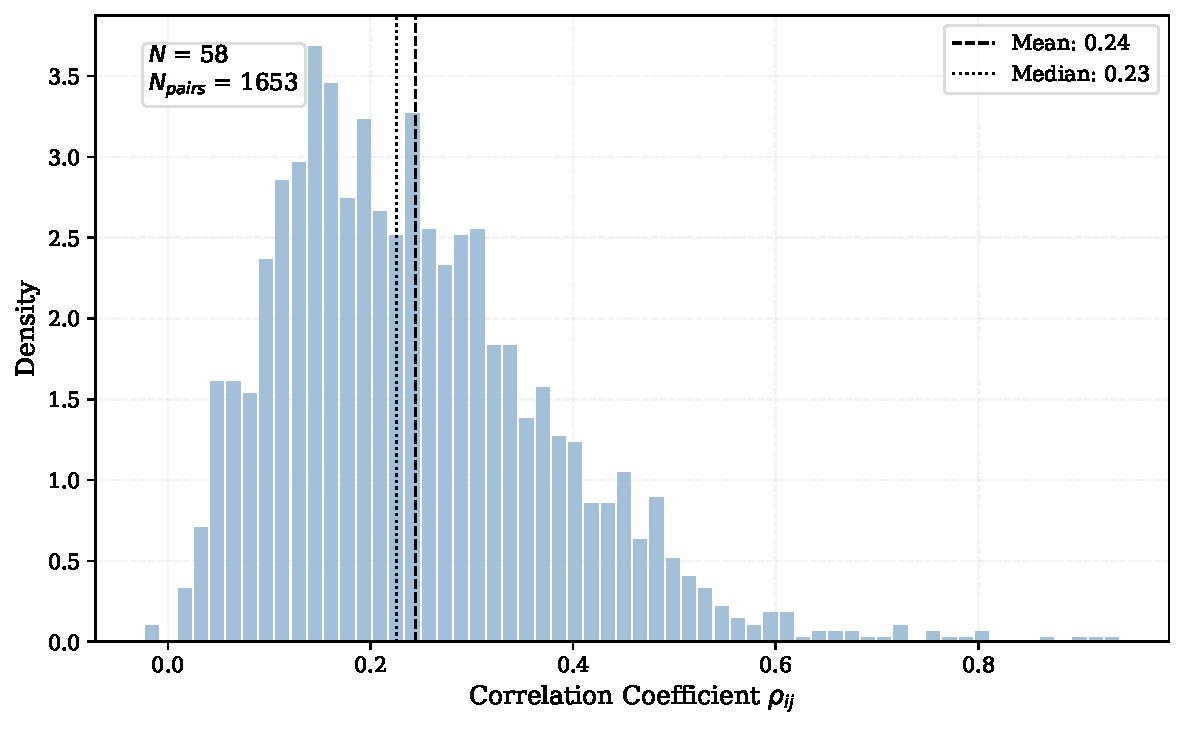
\includegraphics[width=\linewidth]{images/figure_2_correlation_histogram.pdf}
  \vspace{0.2cm}

  \small (a) Full pairwise distribution.
\end{minipage}
\hfill
\begin{minipage}{0.48\linewidth}
  \centering
  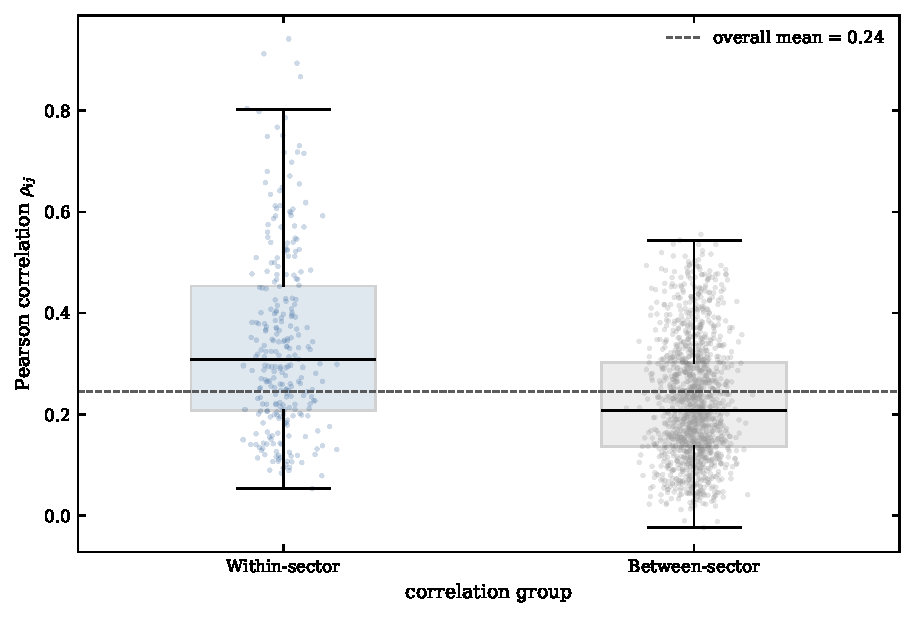
\includegraphics[width=\linewidth]{images/figure_3_sector_correlation_distribution.pdf}
  \vspace{0.2cm}

  \small (b) Within-sector and between-sector pairs.
\end{minipage}

\captionof{figure}{Correlation structure in the core historical universe. Panel (a) shows the full Pearson correlation distribution. Panel (b) compares within-sector and between-sector correlations using the initial macro-sector classification.}
\label{fig:correlation_structure}
\end{center}

\begin{center}
\captionof{table}{Within-sector and between-sector correlation summary.}
\label{tab:sector_corr_summary}
\begin{tabular}{lrrrrrr}
\toprule
Group & Pairs & Mean & Median & Std. dev. & Min & Max \\
\midrule
Within-sector & 275 & 0.3433 & 0.3082 & 0.1819 & 0.0534 & 0.9402 \\
Between-sector & 1378 & 0.2249 & 0.2076 & 0.1166 & -0.0236 & 0.5552 \\
\bottomrule
\end{tabular}
\end{center}


The difference is economically meaningful. Within-sector pairs have mean correlation 0.3433, while between-sector pairs have mean correlation 0.2249, giving $\Delta_{\mathrm{sector}}=0.1184$. An asset-level label-permutation test with 10,000 sector-label reallocations preserves both the observed dependency matrix and the sector-size vector, without treating overlapping pairs as independent observations. None of the permuted statistics reaches the observed difference (null 95th percentile $=0.0245$; one-sided Monte Carlo $p\approx 10^{-4}$, the minimum attainable at this simulation count). The observed difference is also supported by the sector-label permutation analysis reported later in the robustness assessment. At this stage, the relevant result is that the dependency matrix is not characterized solely by homogeneous positive co-movement: stronger relationships are also concentrated within the economic grouping used in the analysis.

The static correlation distribution, however, does not show whether these relationships remain stable through time. We therefore examine selected economically interpretable asset pairs under different dynamic correlation estimators. Figure~\ref{fig:dynamic_pairwise} includes PETR4--VALE3, representing two large commodity-exposed firms in distinct subsectors; BBDC4--BBAS3 in financials; GGBR4--USIM5 in steel and metallurgy; and ELET3--CMIG4 in utilities. These pairs are illustrative rather than intended to represent all possible pairwise relationships.

The pairwise estimates show that individual dependencies can strengthen, weaken, or temporarily break down over time. The 20-day Pearson estimates respond rapidly to local variation, whereas the 60-day estimates provide smoother representations of persistent relationships. The EWMA estimates provide an intermediate view by assigning greater weight to recent observations. The common conclusion across these estimators is that a single full-sample correlation should be interpreted as a long-run summary of an underlying time-varying relationship.

We finally move from individual pairs to market-wide synchronization. Figure~\ref{fig:rolling_corr} reports the average pairwise market correlation estimated with 252- and 504-trading-day rolling windows. Because historical coverage changes in the earliest part of the sample, each window uses the assets available during that period, ranging from approximately 40 assets initially to the complete 58-asset universe in later years. The series should therefore be interpreted as a descriptive measure of average available cross-sectional dependence.

Market-wide correlation varies through time and increases around the 2008 global financial crisis and the 2020 COVID-19 shock. Figure~\ref{fig:rolling_corr} remains close to 0.2 during 2015--2016, so that interval does not show a comparable increase in this measure. These episodes show that the positive dependence observed in the static correlation distribution is not constant through time.

Taken together, the results reveal three complementary features of the B3 dependency structure: positive but heterogeneous cross-sectional correlations, stronger dependence within economic sectors, and substantial variation in synchronization over time. The presence of broad co-movement alongside more localized relationships raises the next question in the empirical sequence: how much of the observed correlation structure is associated with a dominant collective market mode, how much remains in smaller group-level components, and how much is compatible with sampling noise? We address this question next through Random Matrix Theory.

\begin{center}
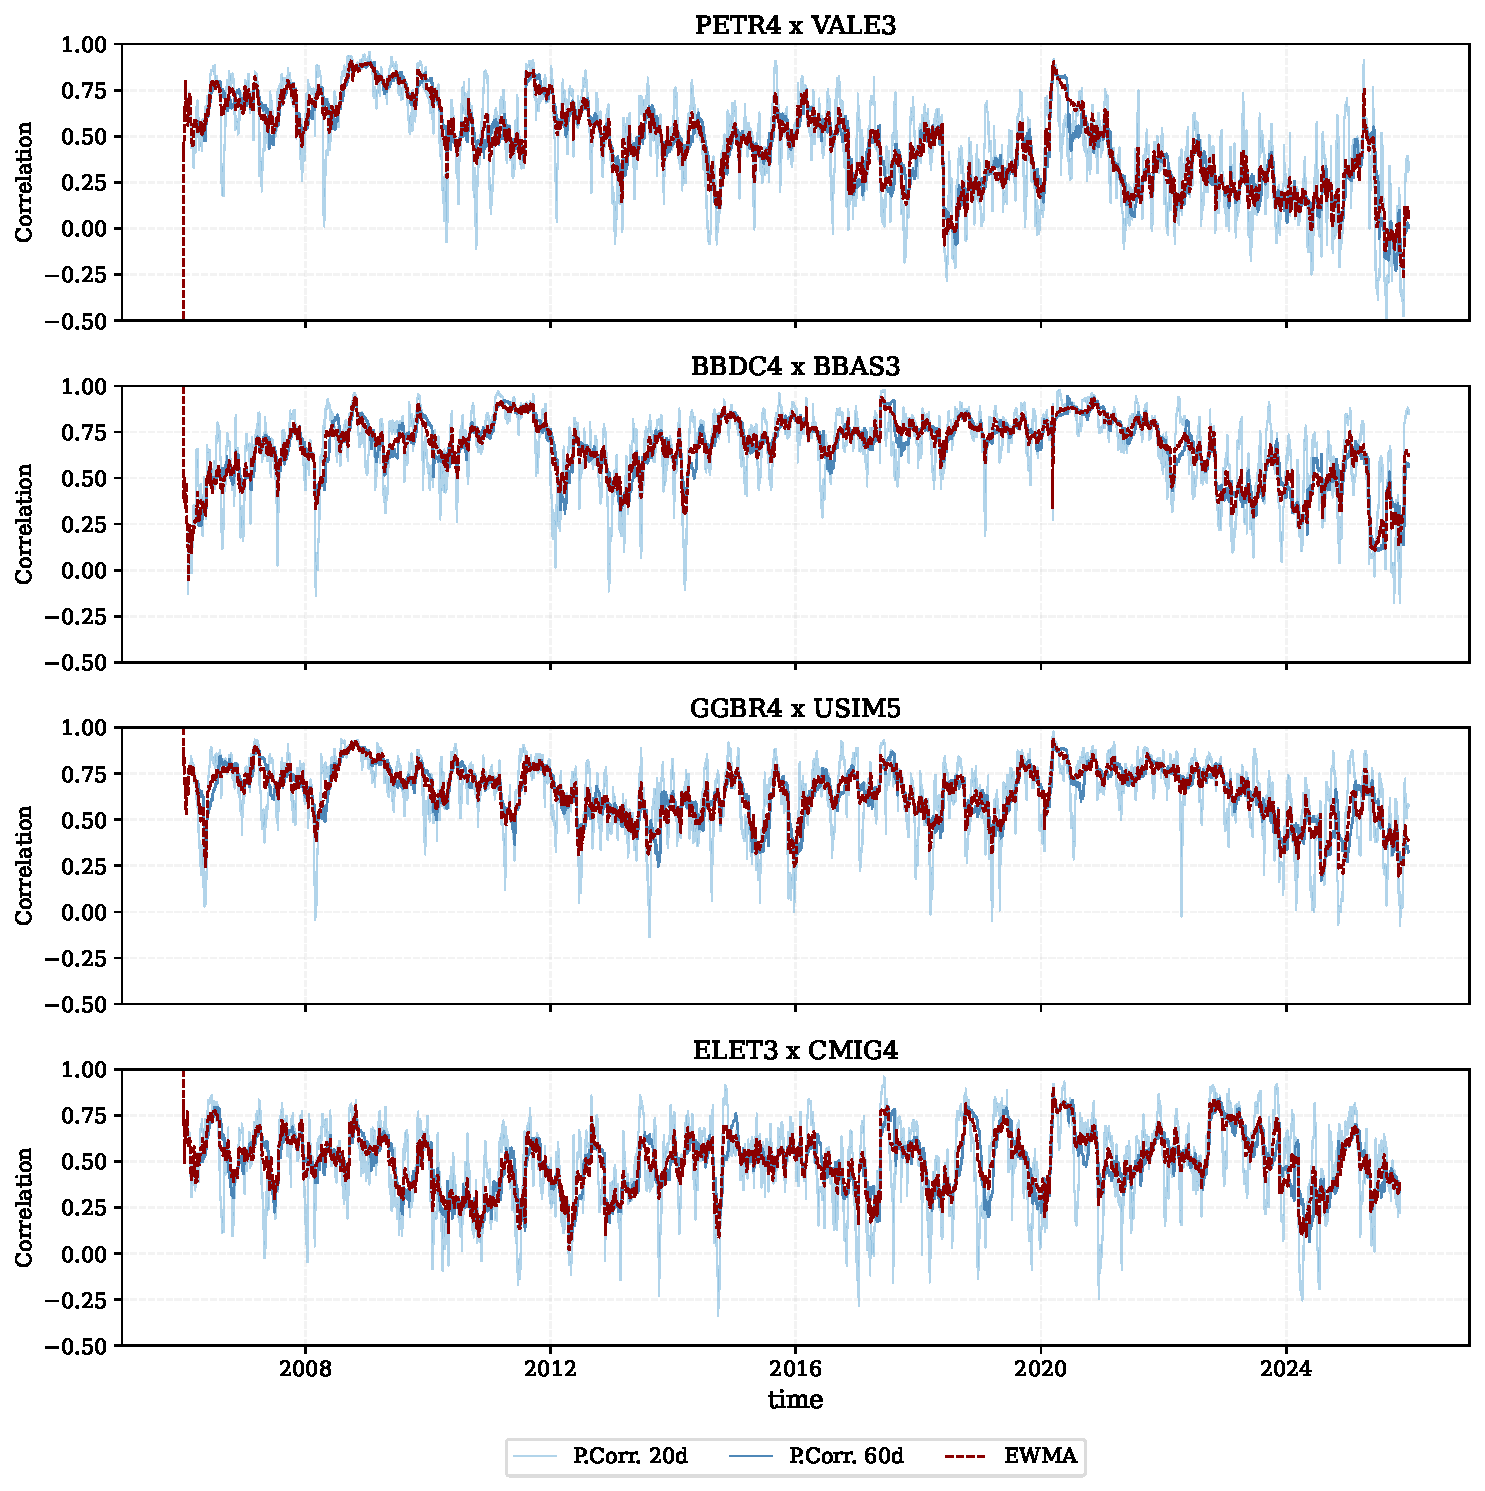
\includegraphics[width=\linewidth]{images/figure_5_dynamic_pairwise_correlations.pdf}
\captionof{figure}{Dynamic pairwise correlations for selected economically interpretable asset pairs. Pearson estimates use 20- and 60-trading-day windows; EWMA uses a 20-day half-life. The estimates show how individual dependencies can vary across time scales.}
\label{fig:dynamic_pairwise}
\end{center}


\begin{center}
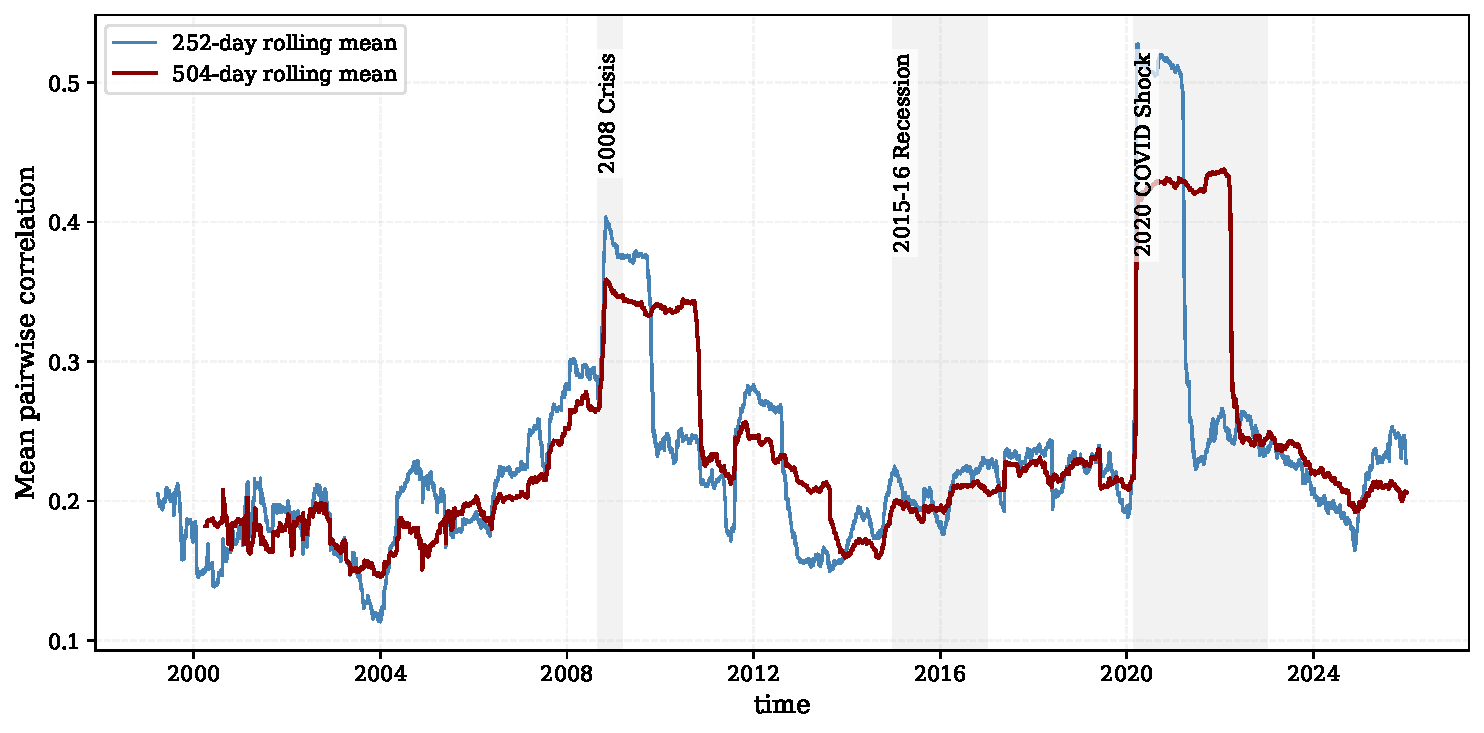
\includegraphics[width=0.95\linewidth]{images/figure_4_rolling_average_correlation.pdf}
\captionof{figure}{Rolling average market correlation for the core historical universe, estimated with 252- and 504-trading-day windows. Each window uses the assets available during that period.}
\label{fig:rolling_corr}
\end{center}


\subsection{Spectral Structure Beyond the Market Mode}
\label{sec:rmt}

The dependence patterns identified in Section~\ref{sec:stylized_correlation} raise a central question: how much of the observed correlation structure reflects broad market synchronization, and how much remains in smaller collective components beyond the sampling-noise benchmark. Following the RMT procedure described in Section~\ref{subsec:rmt_method}, we examine the eigenspectrum of the complete synchronized panel of $N=58$ assets and $T=1527$ observations.

\subsubsection{Empirical Eigenspectrum and Mode Separation
}


For this panel, $Q=T/N=26.33$, yielding Mar\v{c}enko--Pastur bounds of $\lambda_-=0.6482$ and $\lambda_+=1.4278$. Five empirical eigenvalues lie above the upper bound, comprising the market eigenvalue and four additional non-market modes. The mean off-diagonal correlation on this same synchronized $58\times1527$ panel is 0.3350, whereas the leading eigenvalue accounts for 0.3733 of the trace. These are related but distinct summaries: the pairwise mean averages 1,653 correlations, while $\lambda_1/N$ is the leading spectral share and need not equal the mean correlation in a heterogeneous matrix. The approximately 0.24 mean shown for the broader pairwise summaries uses unbalanced pair coverage and a different sample definition.

Table~\ref{tab:rmt_summary} reports the numerical inputs for RMT filtering. The leading eigenvalue, $\lambda_1=21.6505$, is substantially larger than the remaining eigenvalues and accounts for approximately 37.3\% of the total trace of the correlation matrix. The next four eigenvalues, $\lambda_2=3.0957$, $\lambda_3=1.7839$, $\lambda_4=1.6543$, and $\lambda_5=1.4835$, also exceed $\lambda_+$, indicating additional candidate collective structures beyond the dominant market component.

\begin{center}
\captionof{table}{Summary of the RMT eigenspectrum for the complete 58-asset panel.}
\label{tab:rmt_summary}
\setlength{\tabcolsep}{4pt}
\begin{tabular}{rrrrrrr}
\toprule
$N$ & $T$ & $Q$ & $\lambda_-$ & $\lambda_+$ &
Eigenvalues above $\lambda_+$ (total; non-market) & Market-mode share \\
\midrule
58 & 1527 & 26.33 & 0.6482 & 1.4278 & 5 (4) & 37.33\% \\
\bottomrule
\end{tabular}
\end{center}


Figure~\ref{fig:rmt_spectrum} places these eigenvalues against the Mar\v{c}enko--Pastur benchmark. The separation of $\lambda_1$ from both the noise-compatible region and the remaining significant modes provides the first evidence of a dominant collective market component. At the same time, the presence of four additional eigenvalues above $\lambda_+$ indicates that the correlation structure cannot be reduced to market-wide synchronization alone.

The leading eigenvector has positive loadings across the asset universe and therefore represents broad market co-movement. Because this component accounts for approximately 37.3\% of the total trace, it can dominate the structure of the original correlation matrix and obscure weaker localized relationships. We therefore remove the leading mode and reconstruct the component associated with the remaining eigenvalues above the Mar\v{c}enko--Pastur upper bound.

Spectral reconstruction reproduces the original correlation matrix up to floating-point precision, confirming that the subsequent differences between the original and filtered representations arise from the intended mode separation rather than numerical reconstruction error. The complete component-by-component matrix display is provided in supplementary Figure~\ref{fig:rmt_full_components_supplement}; it shows the retained and noise-compatible components that are summarized here.

\begin{center}
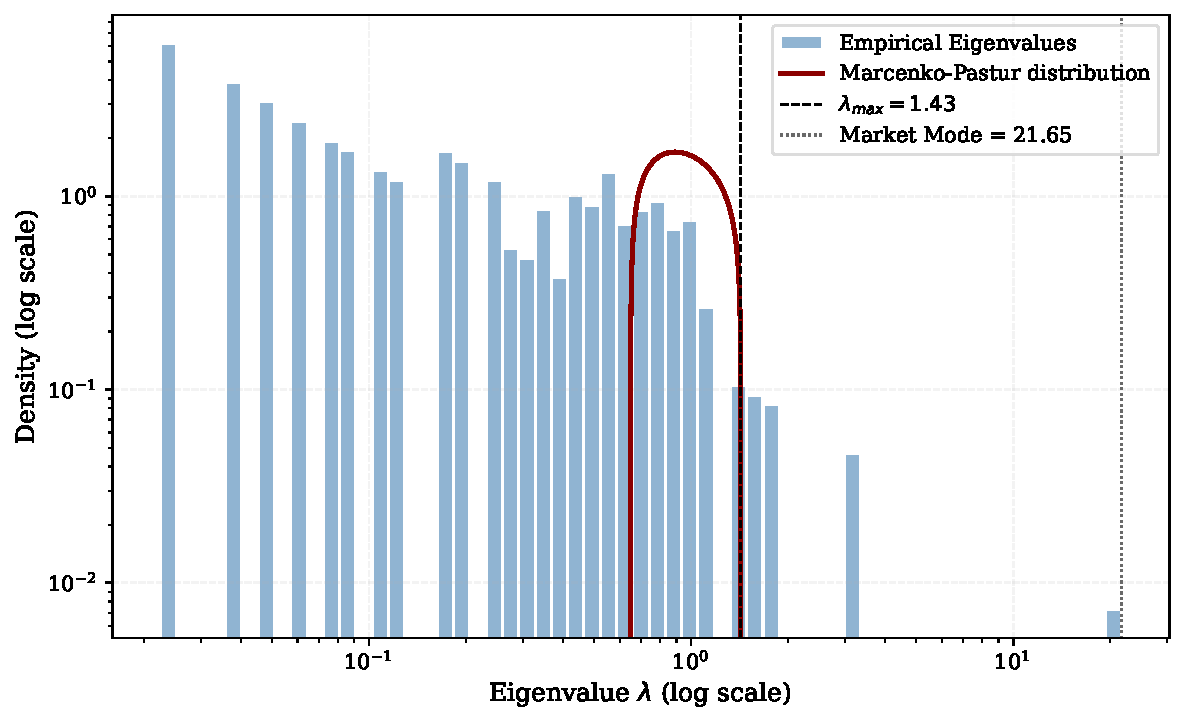
\includegraphics[width=0.85\linewidth]{images/figure_6_rmt_eigenvalue_spectrum.pdf}
\captionof{figure}{Empirical eigenvalue spectrum and Mar\v{c}enko--Pastur bounds. The largest eigenvalue is far outside the random band and captures the market-mode component.}
\label{fig:rmt_spectrum}
\end{center}

Figure~\ref{fig:rmt_filtered_matrices} shows the effect of this separation. The original matrix is dominated by broadly positive correlations, consistent with the strong collective component identified in the eigenspectrum. After removal of the leading mode, the candidate group-mode component reveals a more heterogeneous pattern, with localized positive and negative contrasts that were less visible in the original matrix.
\begin{center}
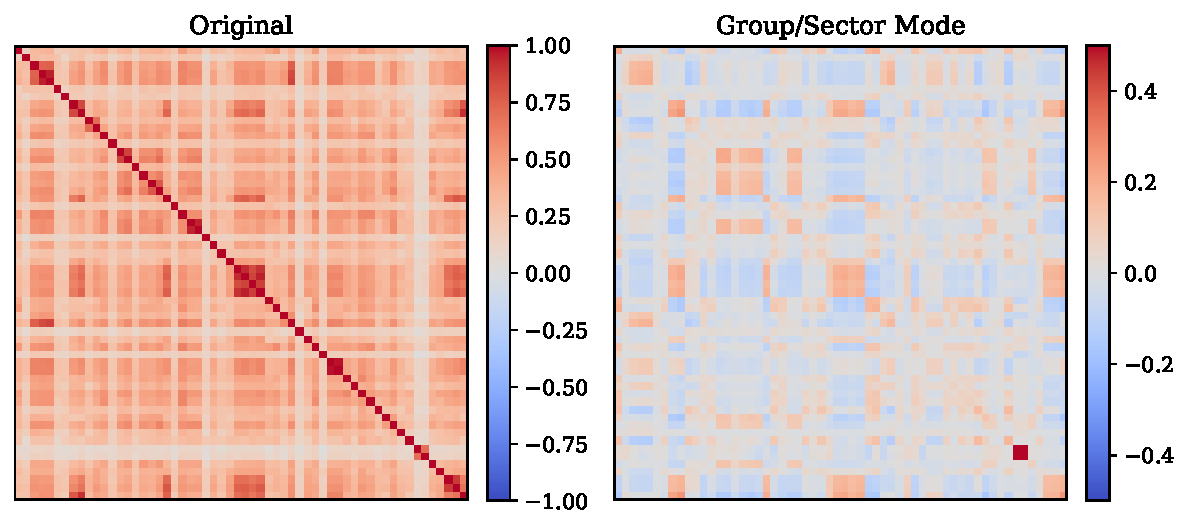
\includegraphics[width=0.9\linewidth]{images/figure_8_original_group_matrices.pdf}
\captionof{figure}{Original and candidate group-mode RMT component matrices at readable scale. The original matrix is dominated by broad positive co-movement, whereas the group-mode component highlights weaker localized contrasts after the leading market mode is removed.}
\label{fig:rmt_filtered_matrices}
\end{center}

The persistence of structured contrasts after market-mode removal suggests that the significant non-leading modes are not merely weaker copies of the collective component. Their composition must therefore be examined directly through their eigenvector loadings before determining whether the same organization reappears in hierarchical and network representations.

\subsubsection{Composition of the Significant Spectral Modes}

Eigenvalues indicate the strength of collective modes, while their eigenvectors reveal how individual assets contribute to each component. Figure~\ref{fig:eigenvector_loadings} reports the largest loadings for the five eigenvalues above the Mar\v{c}enko--Pastur upper bound. Assets are ranked by loading magnitude within each eigenvector. Because the overall sign of an eigenvector is arbitrary, the interpretation focuses on the relative contrasts, magnitude, and concentration of the loadings.

\begin{center}
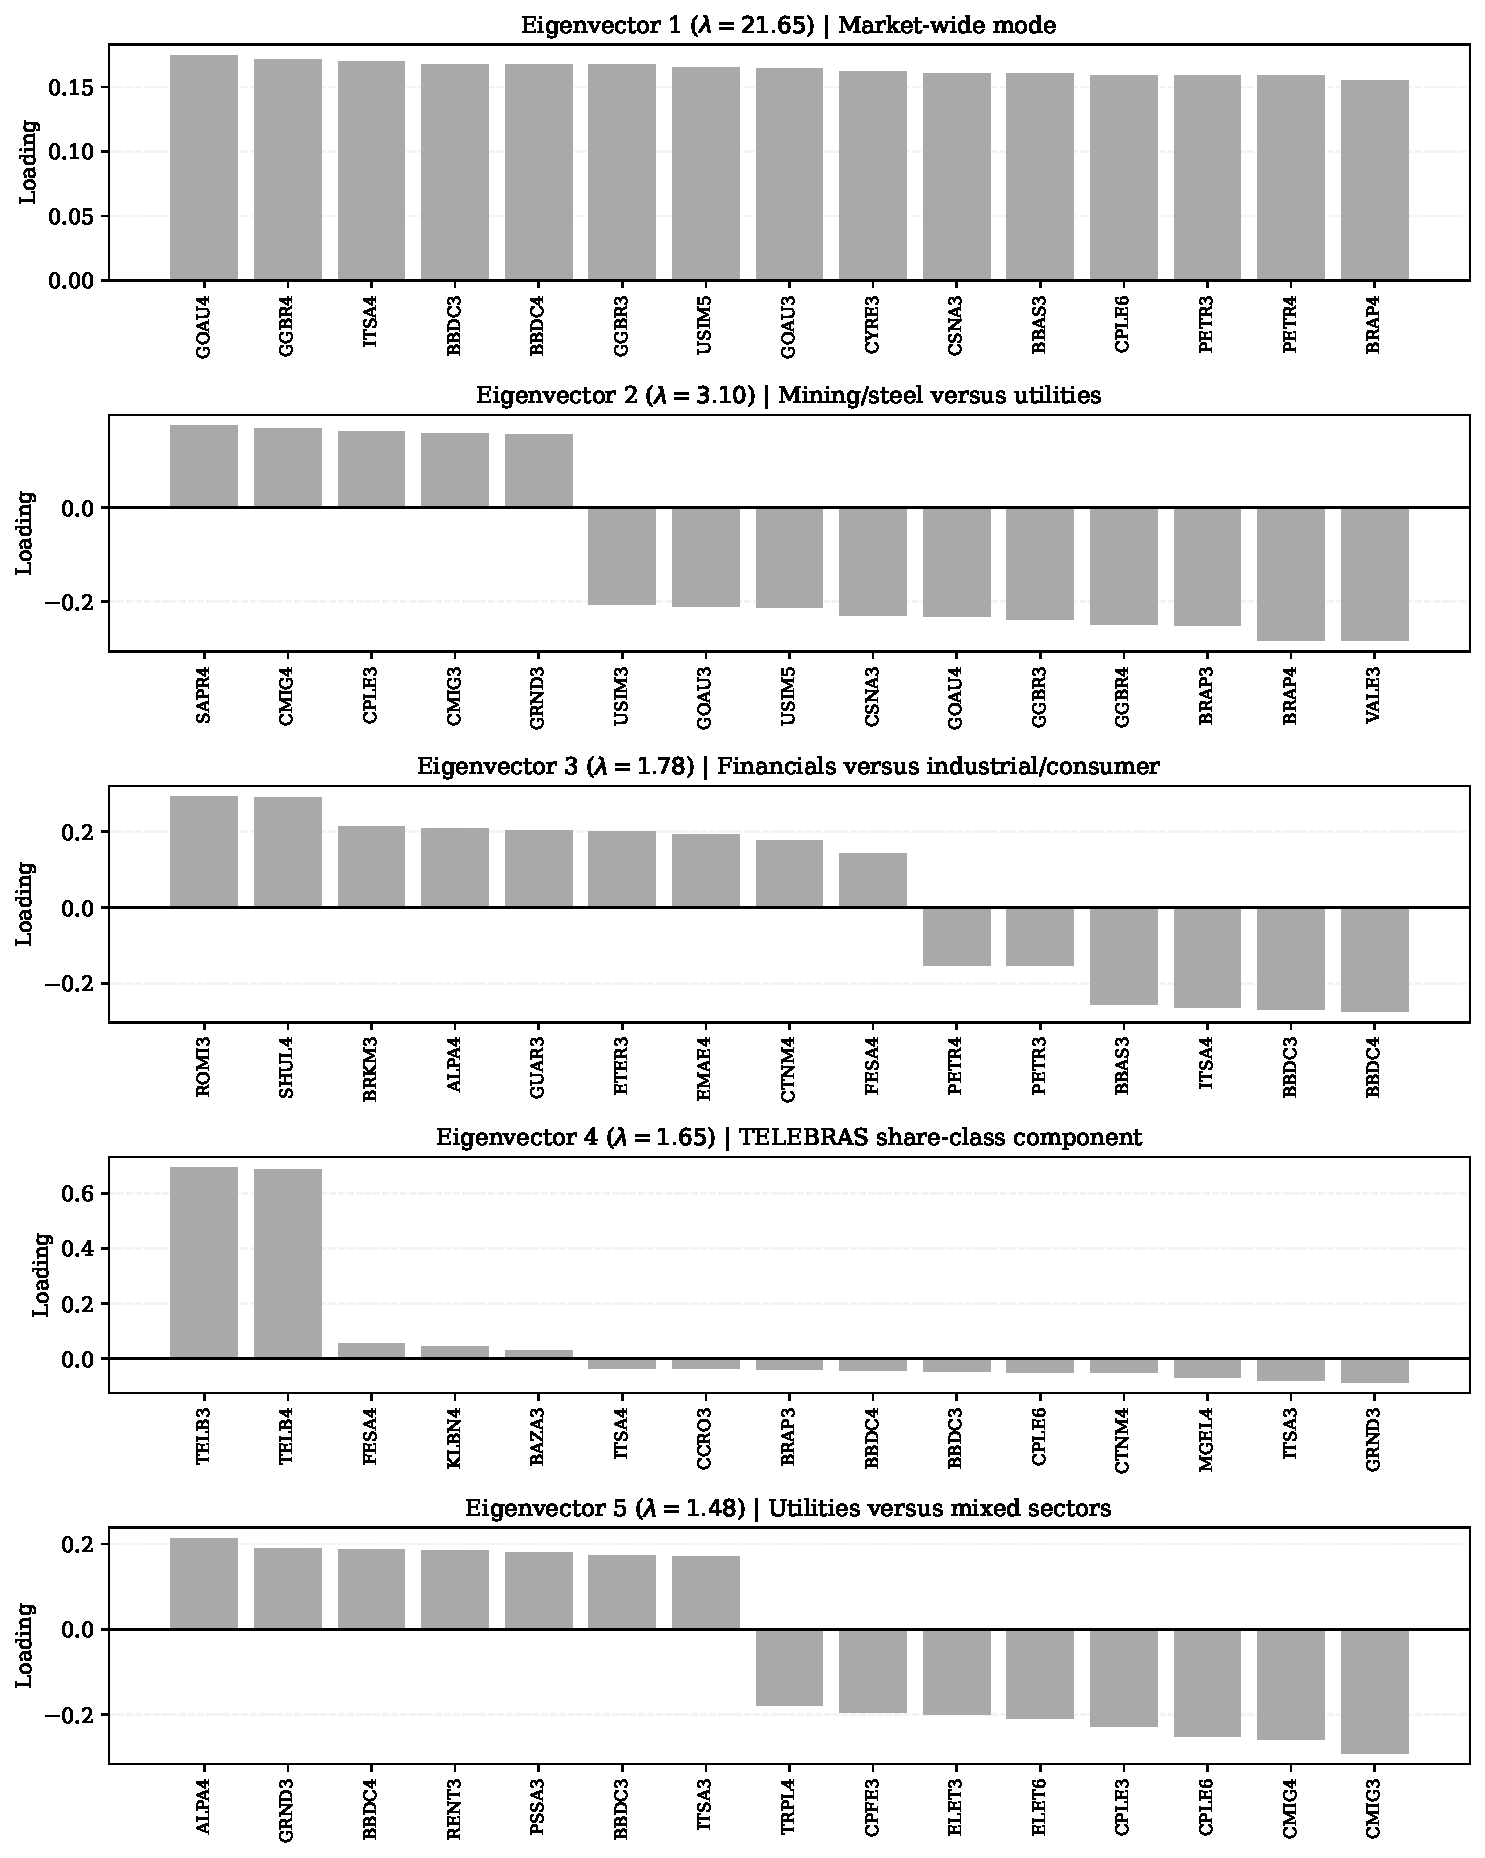
\includegraphics[width=0.95\linewidth]{images/figure_7b_rmt_top_eigenvectors_top_loadings.pdf}
\captionof{figure}{Top eigenvector loadings for the five RMT modes above the Mar\v{c}enko--Pastur upper bound. Eigenvector 1 is a broad market mode. Subsequent eigenvectors show relative contrasts between groups of assets; their overall signs are arbitrary.}
\label{fig:eigenvector_loadings}
\end{center}

The first eigenvector exhibits positive loadings across all 58 assets, ranging from 0.037 to 0.174. Its contribution is distributed across multiple sectors rather than concentrated in a single economic group, reinforcing the interpretation of the leading component as a broad market mode.

The second eigenvector ($\lambda_2=3.10$) is best read as a relative contrast between mining and steel firms---including VALE3, BRAP3/4, GGBR3/4, GOAU3/4, CSNA3 and USIM3/5---and a group led by utilities and selected consumer-cyclical assets. It therefore contains a commodity-related dimension, but it is not a pure Basic Materials factor.

The third eigenvector ($\lambda_3=1.78$) similarly contrasts the financial pole formed by BBDC3/4, ITSA4 and BBAS3 with a more heterogeneous industrial, chemical and consumer-cyclical pole led by ROMI3, SHUL4, BRKM3, ALPA4 and GUAR3.

The fourth eigenvector ($\lambda_4=1.65$) is highly concentrated in TELB3 and TELB4, the two listed TELEBRAS share classes. We interpret this result as an issuer-specific share-class component, rather than as evidence of a broad telecommunications factor. 

The fifth eigenvector ($\lambda_5=1.48$) separates a coherent utilities block---including CEMIG, COPEL, Eletrobras, CPFL Energia and ISA CTEEP---from financial and selected consumer-cyclical assets. This is a plausible utilities-related pattern, but $\lambda_5$ lies only about 3.7\% above the Mar\v{c}enko--Pastur upper bound. Its economic interpretation should therefore remain cautious and be treated as a candidate localized mode.

Overall, Figure~\ref{fig:eigenvector_loadings} shows that the modes beyond the dominant market component are structured contrasts rather than simple one-sector classifications. Some modes align partially with recognizable economic groups, while others reflect more localized or issuer-specific relationships. This motivates the subsequent hierarchical and network analyses, which examine whether these spectral patterns reappear in alternative representations of the dependency structure.


\subsection{Hierarchical and Network Organization After Spectral Filtering}
\label{sec:network_organization}

The spectral analysis in Section~\ref{sec:rmt} showed that removing the dominant market mode reveals weaker but structured dependencies among groups of assets. We now examine whether these patterns also appear in the distance geometry of the correlation matrices. Hierarchical ordering provides a complementary representation of the same dependency structure, allowing localized organization to be compared across the original and RMT-filtered matrices.

\subsubsection{Hierarchical Organization of the Filtered Dependence Structure}
\label{sec:clustering}

Figure~\ref{fig:ordered_heatmaps} shows the correlation matrices after hierarchical ordering. The original matrix retains a broad positive background, consistent with the dominant collective component identified in the eigenspectrum. After spectral filtering, this common background is reduced and localized blocks become more visible. The group-mode representation is particularly informative because it emphasizes relative dependencies that remain after removal of the leading market component.

\begin{center}
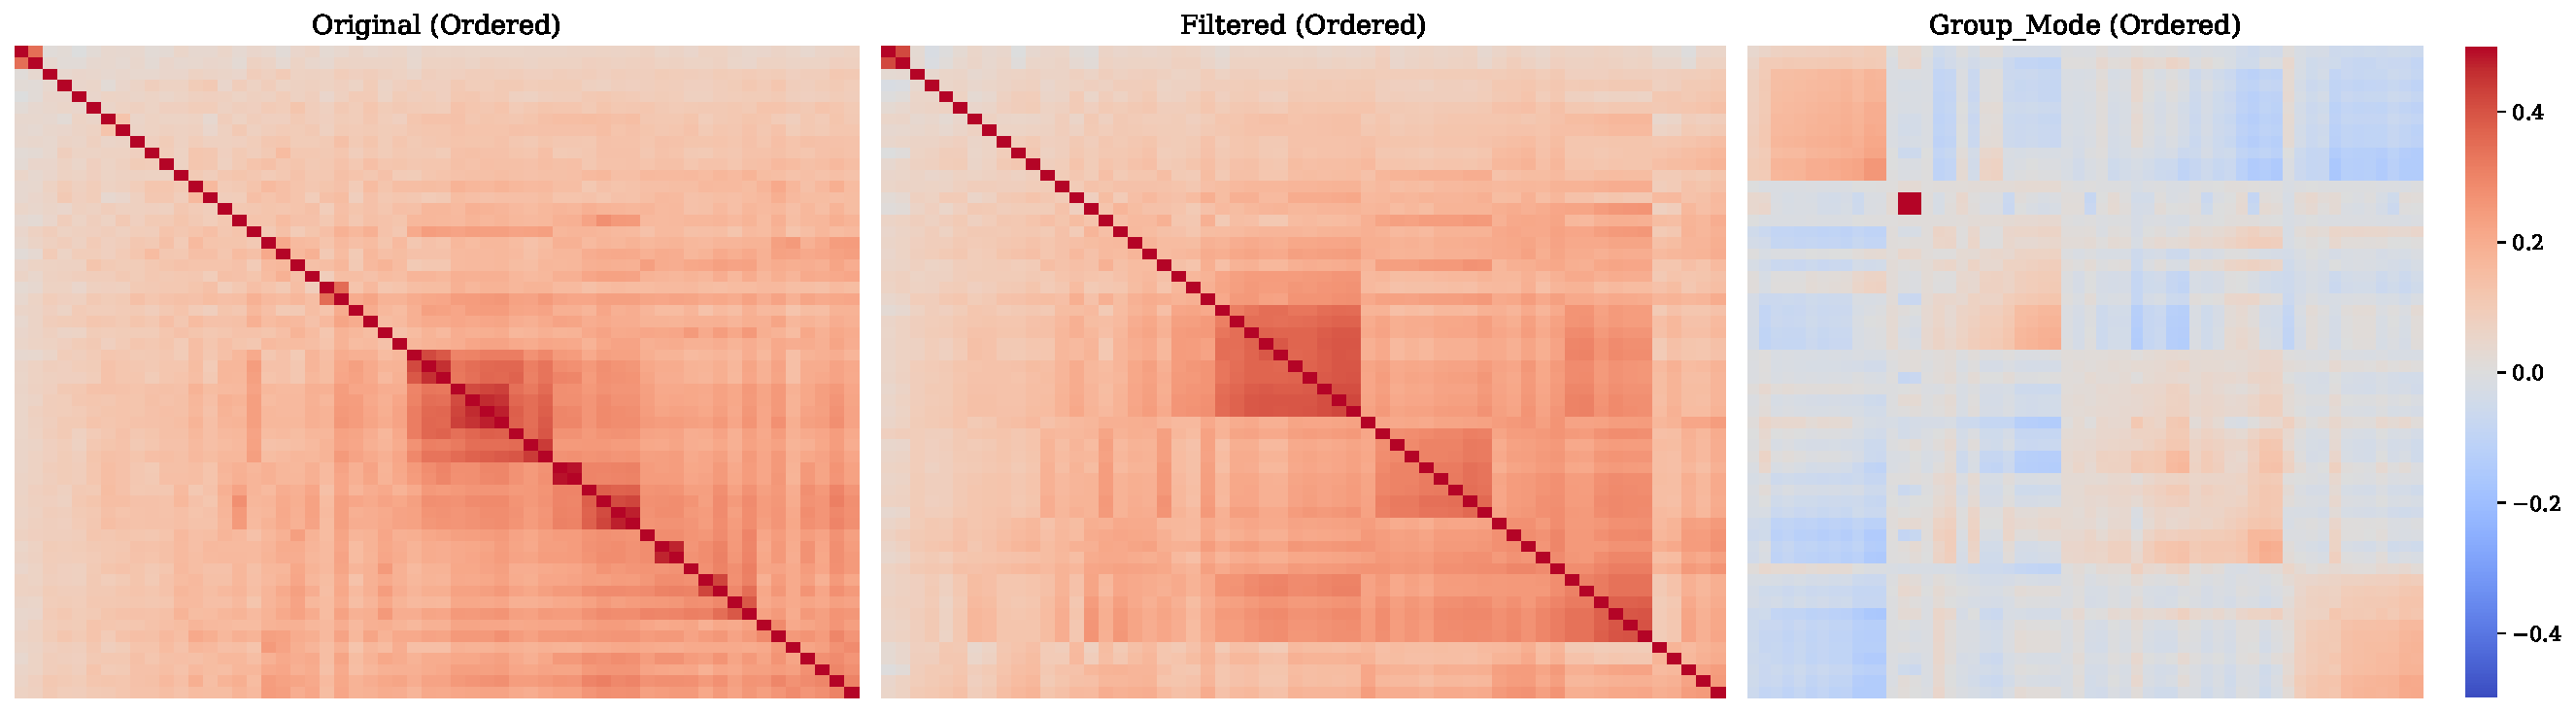
\includegraphics[
width=\linewidth,
height=0.72\textheight,
keepaspectratio
]{images/figure_10_ordered_heatmaps.pdf}
\captionof{figure}{Hierarchically ordered correlation matrices for the original and RMT-filtered structures. The common color scale highlights the reduction of broad market-wide co-movement and the emergence of more localized dependency patterns after spectral filtering.}
\label{fig:ordered_heatmaps}
\end{center}

The ordered matrices indicate that market-mode removal does not eliminate organization from the dependency structure. Instead, it changes its scale: the broad positive background becomes weaker while smaller blocks of relatively stronger and weaker relationships become easier to distinguish. These patterns are consistent with the heterogeneous compositions observed in the non-leading eigenvectors and suggest that part of the residual spectral structure is also expressed geometrically.

The corresponding hierarchical tree provides a more compact view of this organization. Figure~\ref{fig:dendrograms} shows the group-mode dendrogram obtained from Mantegna distances and average linkage. To shorten the long horizontal branches, the plotted merge heights use a monotone logarithmic transform; the tick labels report the original distances. Macro-sector colors are included only as an external reference for interpretation; the clustering procedure itself does not impose sector labels.

\begin{center}
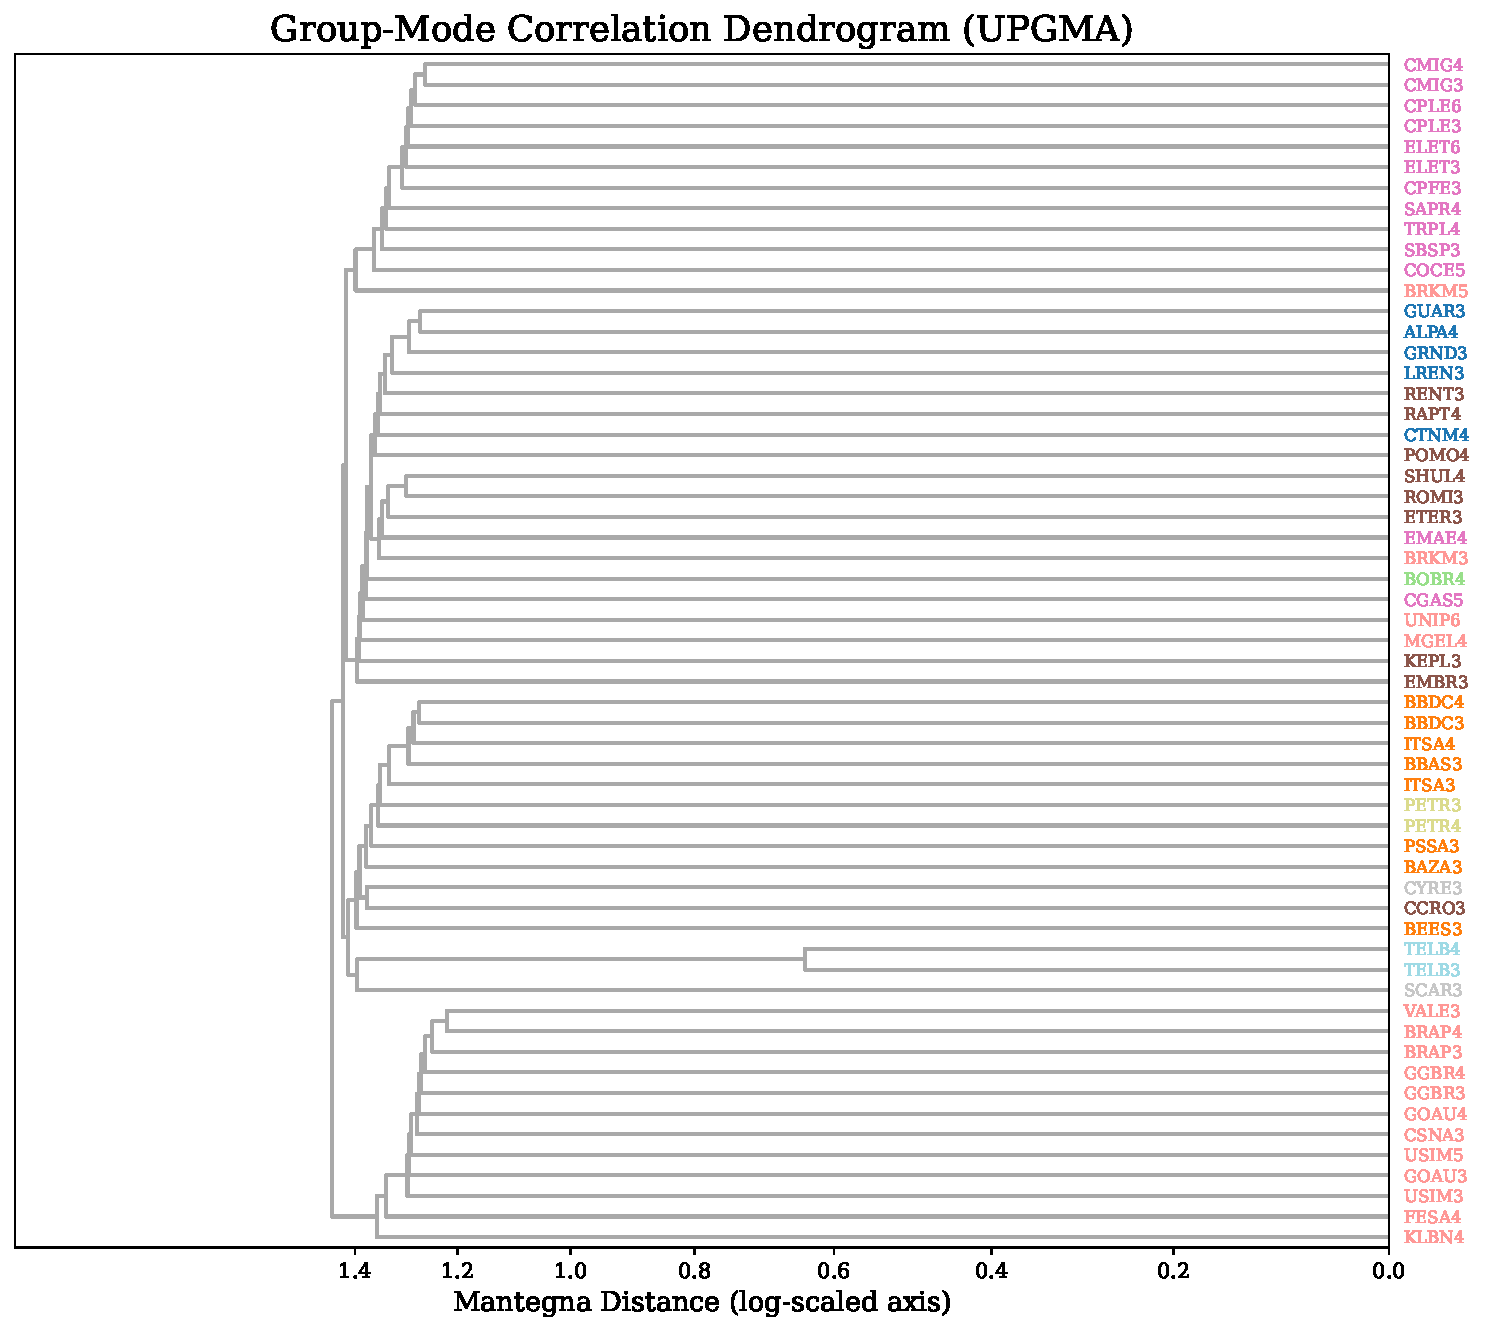
\includegraphics[
width=0.82\linewidth,
height=0.8\textheight,
keepaspectratio
]{images/figure_9_group_mode_dendrogram.pdf}
\captionof{figure}{Group-mode dendrogram obtained from Mantegna distances and average linkage. The horizontal axis uses a monotone log transformation, with tick labels in the original distance scale. The tree summarizes the dependency geometry remaining after removal of the dominant market mode; label colors indicate the initial macro-sector classification for comparison.}
\label{fig:dendrograms}
\end{center}

Table~\ref{tab:cophenetic_summary} compares how closely the hierarchical trees preserve the underlying distance structures.

\begin{center}
\captionof{table}{Cophenetic correlations for the original and RMT-filtered dependency structures.}
\label{tab:cophenetic_summary}
\begin{tabular}{lrr}
\toprule
Matrix & Assets & Cophenetic correlation \\
\midrule
Original & 58 & 0.950 \\
Filtered & 58 & 0.934 \\
Group-mode & 58 & 0.871 \\
\bottomrule
\end{tabular}
\end{center}


The supplementary Figure~\ref{fig:dendrograms_full_supplement} compares the original, filtered and group-mode trees side by side; it shows the additional geometric context for the focused group-mode tree in Figure~\ref{fig:dendrograms}. The original matrix has the highest cophenetic correlation, at 0.950, followed by the filtered matrix at 0.934 and the group-mode matrix at 0.871. The decline after market-mode removal indicates that the residual dependency structure is less accurately represented by a strictly hierarchical tree. This does not imply the disappearance of localized organization; rather, it suggests that the remaining geometry is more complex than the broad market-dominated structure observed in the original matrix.

The hierarchical analysis therefore provides two complementary findings. First, localized dependency patterns remain visible after removal of the dominant market component. Second, these relationships become less purely tree-like as the common market structure is removed. This motivates moving from hierarchical representations to graph-based filtering, where additional connections can be retained and the reorganization of hubs, local connectivity, and sectoral relationships can be examined directly.


\subsubsection{Network Topology Before and After Market-Mode Removal}
\label{sec:networks}

The hierarchical analysis showed that localized dependency patterns remain after removal of the dominant market component, although the resulting geometry becomes less purely tree-like. We therefore move to graph-based representations, which retain selected dependency links and allow changes in connectivity, local organization, and centrality to be examined directly. We compare networks constructed from the original correlation matrix with those obtained from the group-mode component identified through RMT.

The Minimum Spanning Tree (MST) provides the sparsest connected representation of the dependency structure. With $N=58$ assets, each MST contains 57 edges. Figure~\ref{fig:mst_refined} compares the original and group-mode backbones.

\begin{center}
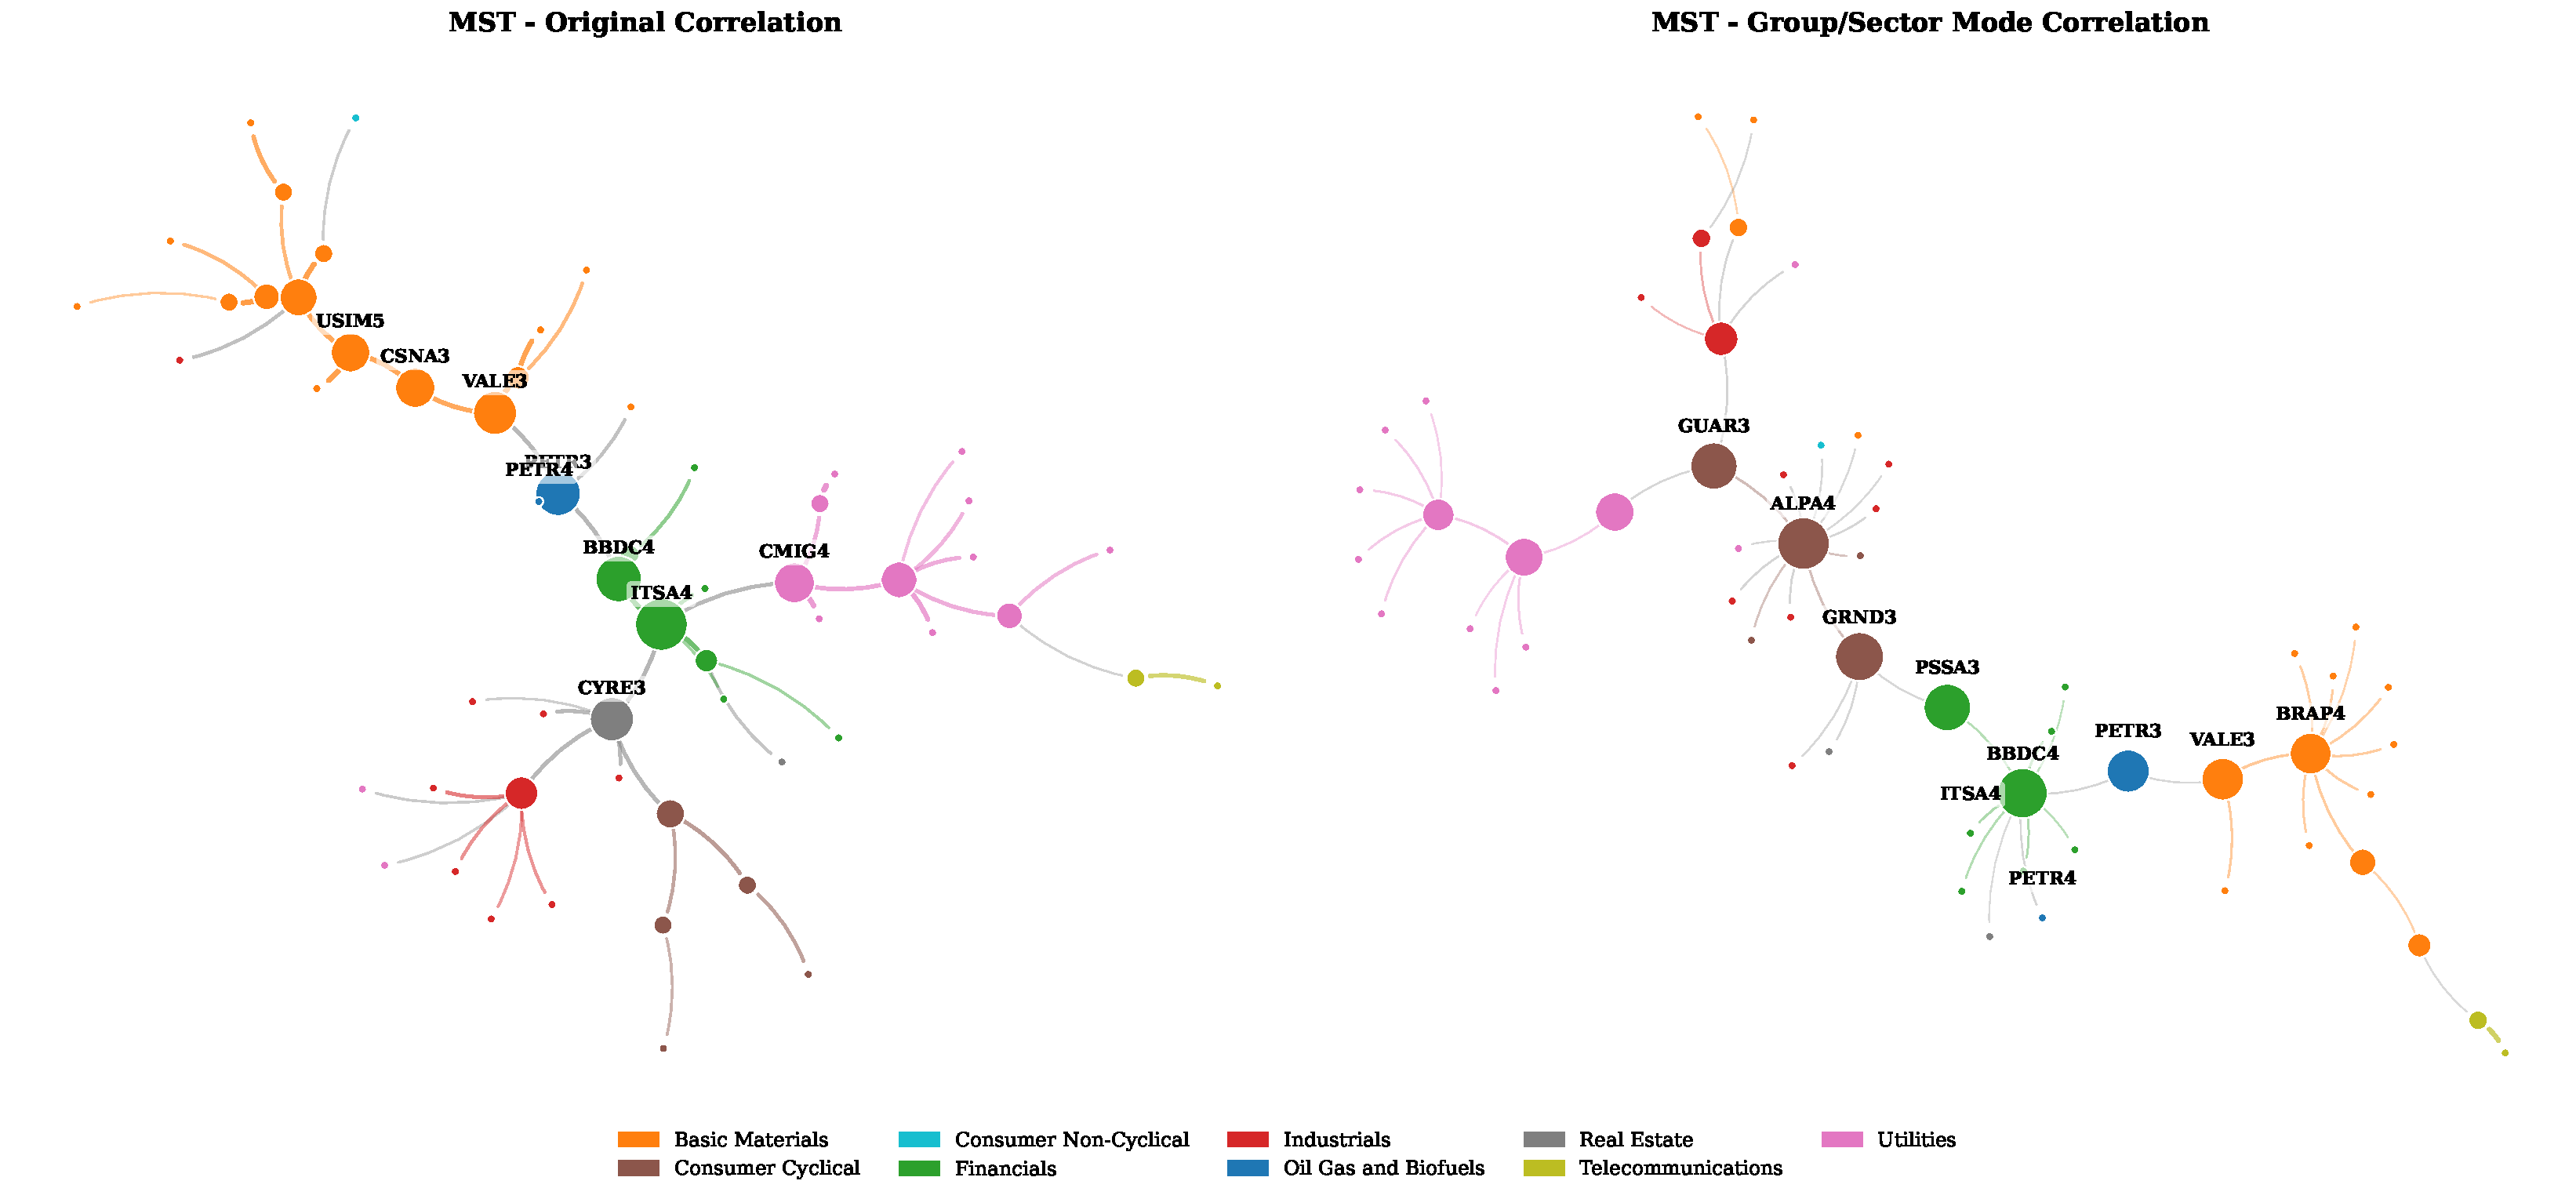
\includegraphics[
width=\linewidth,
height=0.58\textheight,
keepaspectratio
]{images/figure_11b_mst_refined_comparison.pdf}
\captionof{figure}{MST comparison for the original and group-mode correlation structures. Removal of the dominant market component changes the set of strongest dependency channels retained in the network backbone.}
\label{fig:mst_refined}
\end{center}

The original MST has a mean edge correlation of 0.5796, compared with 0.1388 for the group-mode MST. This reduction is expected because the latter excludes the dominant common component. More importantly, the same-sector edge ratio decreases from 0.7193 to 0.6316, indicating that the topology is reorganized rather than simply weakened. The group-mode MST therefore represents a different dependency backbone, emphasizing relationships that remain after broad market synchronization is removed.

The Planar Maximally Filtered Graph (PMFG) provides a richer representation of the same dependency geometry. Unlike the MST, the PMFG retains $3N-6=168$ edges and allows cycles, triangles, and cliques to remain in the graph. Figure~\ref{fig:pmfg_refined} compares the original and group-mode PMFGs.

\begin{center}
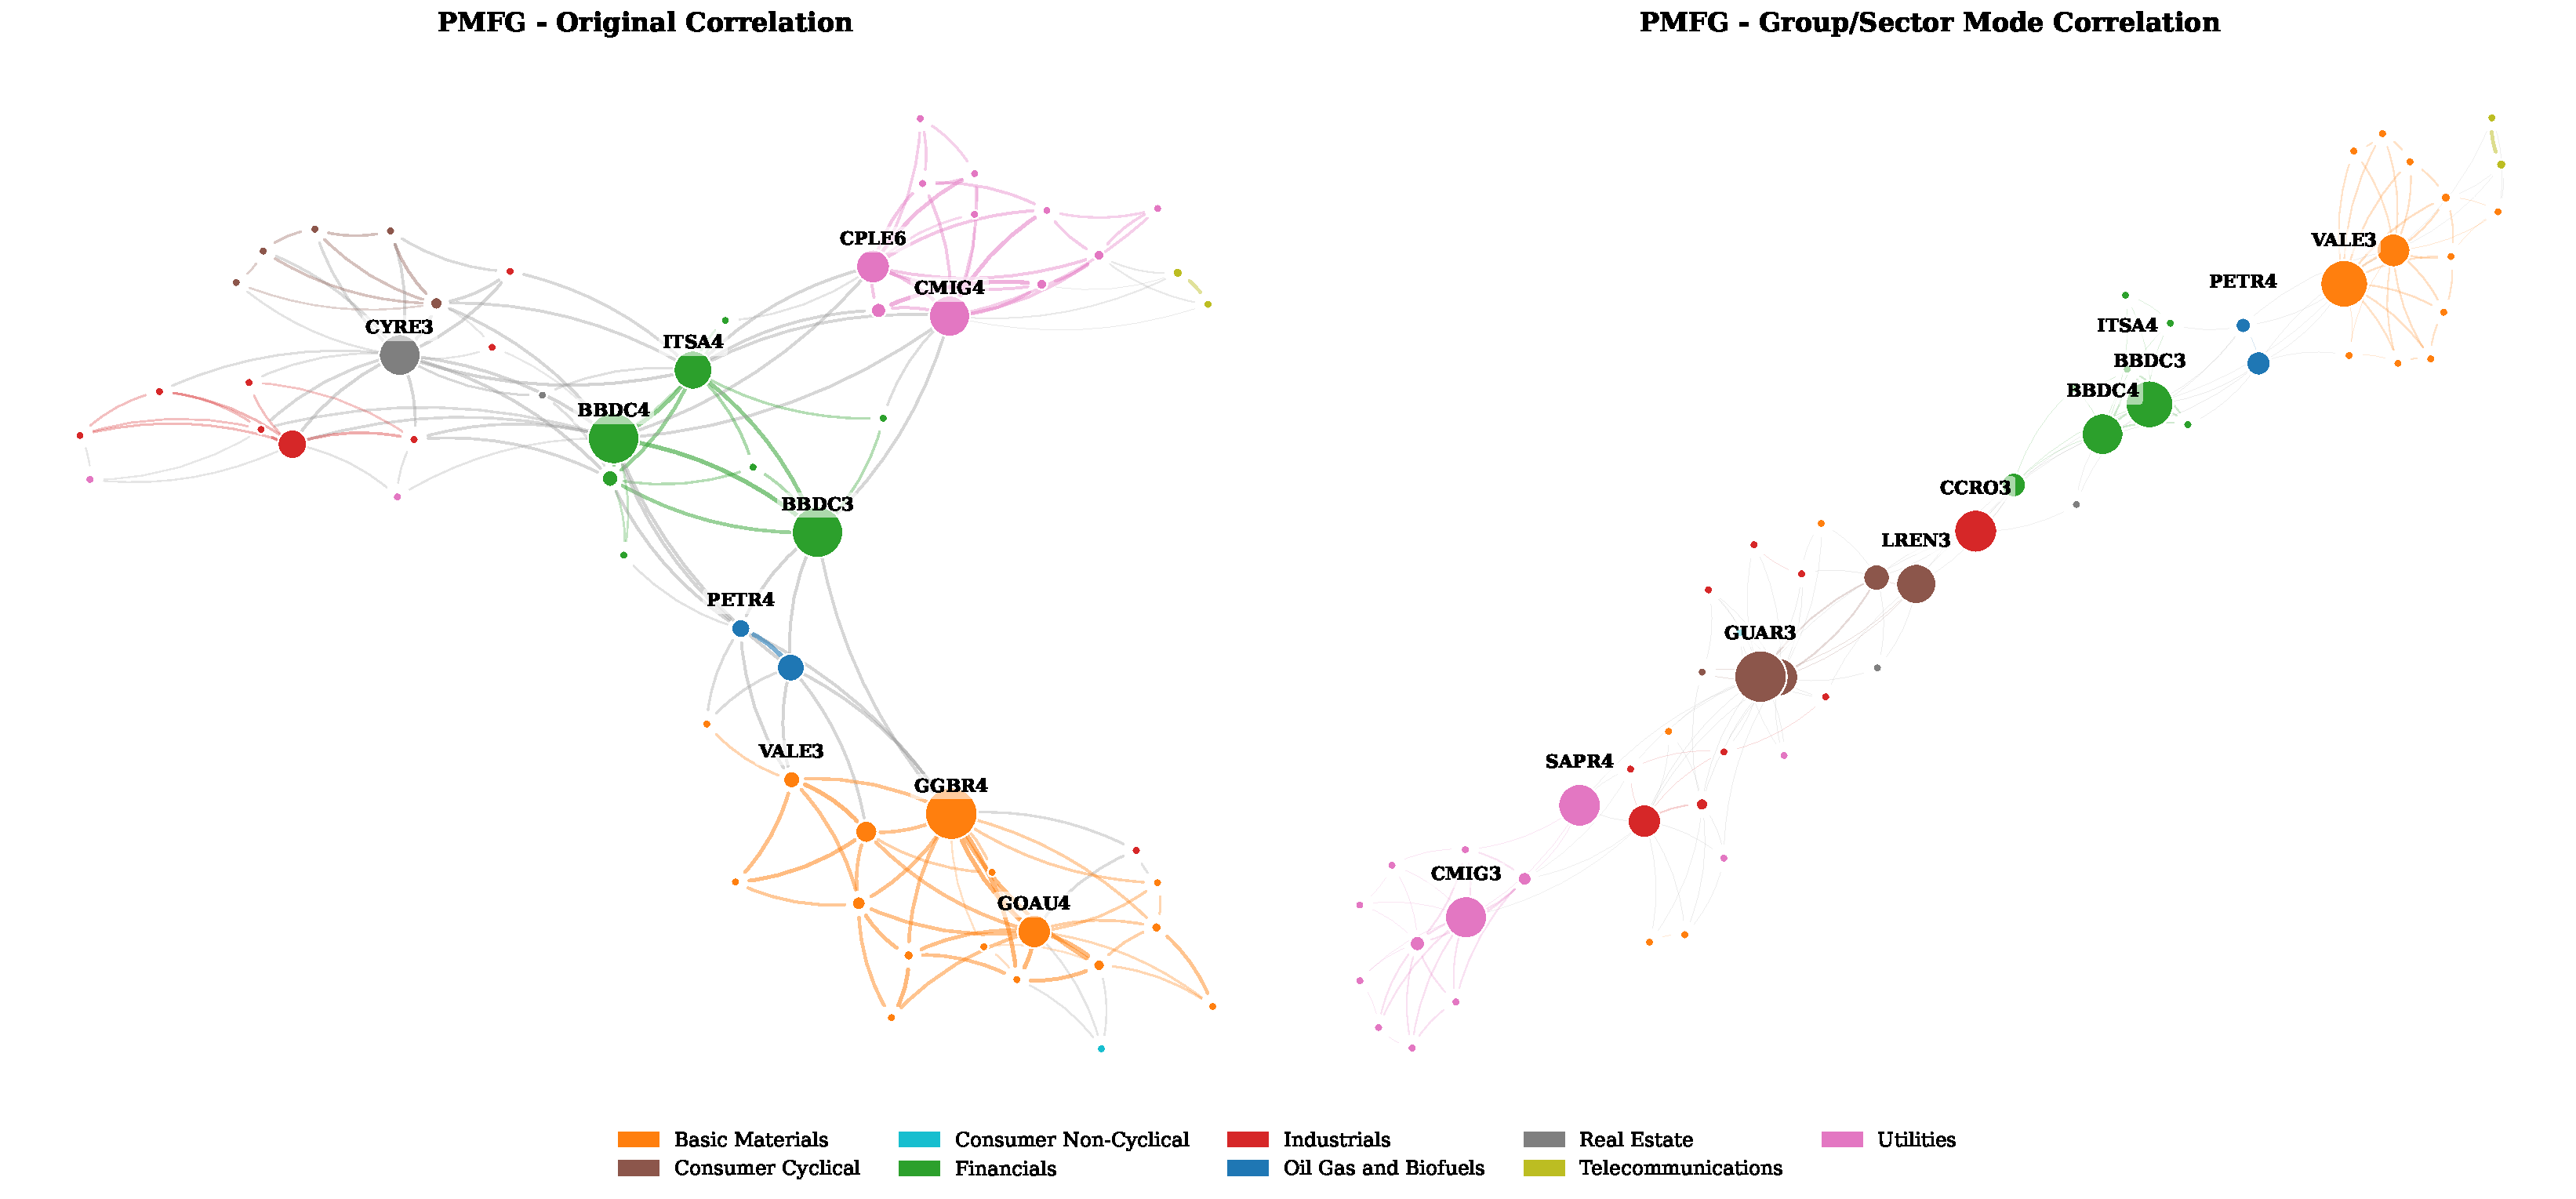
\includegraphics[
width=\linewidth,
height=0.58\textheight,
keepaspectratio
]{images/figure_12b_pmfg_refined_comparison.pdf}
\captionof{figure}{PMFG comparison for the original and group-mode correlation structures. The group-mode representation removes broad market-wide dominance while retaining a denser set of localized dependency relationships.}
\label{fig:pmfg_refined}
\end{center}

As in the MST, average edge strength decreases substantially after market-mode removal, from 0.5177 in the original PMFG to 0.1109 in the group-mode PMFG. The topological response, however, is not a uniform loss of structure. Average clustering increases from 0.5273 to 0.6653, while the same-sector edge ratio decreases from 0.6012 to 0.5417. Thus, weaker absolute correlations coexist with stronger local triangular organization after removal of the broad market component.

Table~\ref{tab:network_summary} summarizes the main differences across the two graph families.

\begin{center}
\captionof{table}{Selected topology statistics for the original and group-mode MST and PMFG representations.}
\label{tab:network_summary}
\small
\setlength{\tabcolsep}{3.5pt}
\begin{tabular}{llrrrrrr}
\toprule
Network & Matrix & Edges & Mean corr. & Same-sector & Clustering & Top degree & Top betweenness \\
\midrule
MST & Original & 57 & 0.5796 & 0.7193 & 0.0000 & RAPT4 & ITSA4 \\
MST & Group mode & 57 & 0.1388 & 0.6316 & 0.0000 & ALPA4 & ALPA4 \\
PMFG & Original & 168 & 0.5177 & 0.6012 & 0.5273 & BBDC4 & GGBR4 \\
PMFG & Group mode & 168 & 0.1109 & 0.5417 & 0.6653 & GUAR3 & GUAR3 \\
\bottomrule
\end{tabular}
\end{center}


The comparison reveals a consistent pattern across MST and PMFG representations. Removing the dominant market mode substantially reduces edge strength and partially reduces sectoral concentration, but it does not eliminate organized dependency structure. In the PMFG, the simultaneous reduction in average correlation and increase in clustering is particularly informative: the residual network is weaker in absolute correlation terms but more locally organized around interconnected groups of assets.

The PMFG construction also retains the expected planar structure, with 168 edges, 166 triangles, and 55 four-cliques for the 58-asset network. These quantities are primarily construction diagnostics and are therefore reported in detail in the supplementary material. Their main role here is to confirm that the PMFG preserves local structures that cannot appear in the MST. The remaining question is whether removal of the market mode also changes which assets occupy structurally important positions. We therefore examine hub reorganization next.


\subsubsection{Hub Reorganization and Subsector-Level Dependencies}
\label{sec:subsector_network}

The changes observed in MST and PMFG topology are also reflected in the identity of the most central assets. Figure~\ref{fig:hub_rank} compares hub rankings before and after removal of the dominant market mode. In the original PMFG, BBDC4 has the highest degree and GGBR4 the highest betweenness, whereas GUAR3 becomes the leading node according to both measures in the group-mode network. The change indicates that centrality depends strongly on whether broad market co-movement is retained in the underlying correlation structure.

\begin{center}
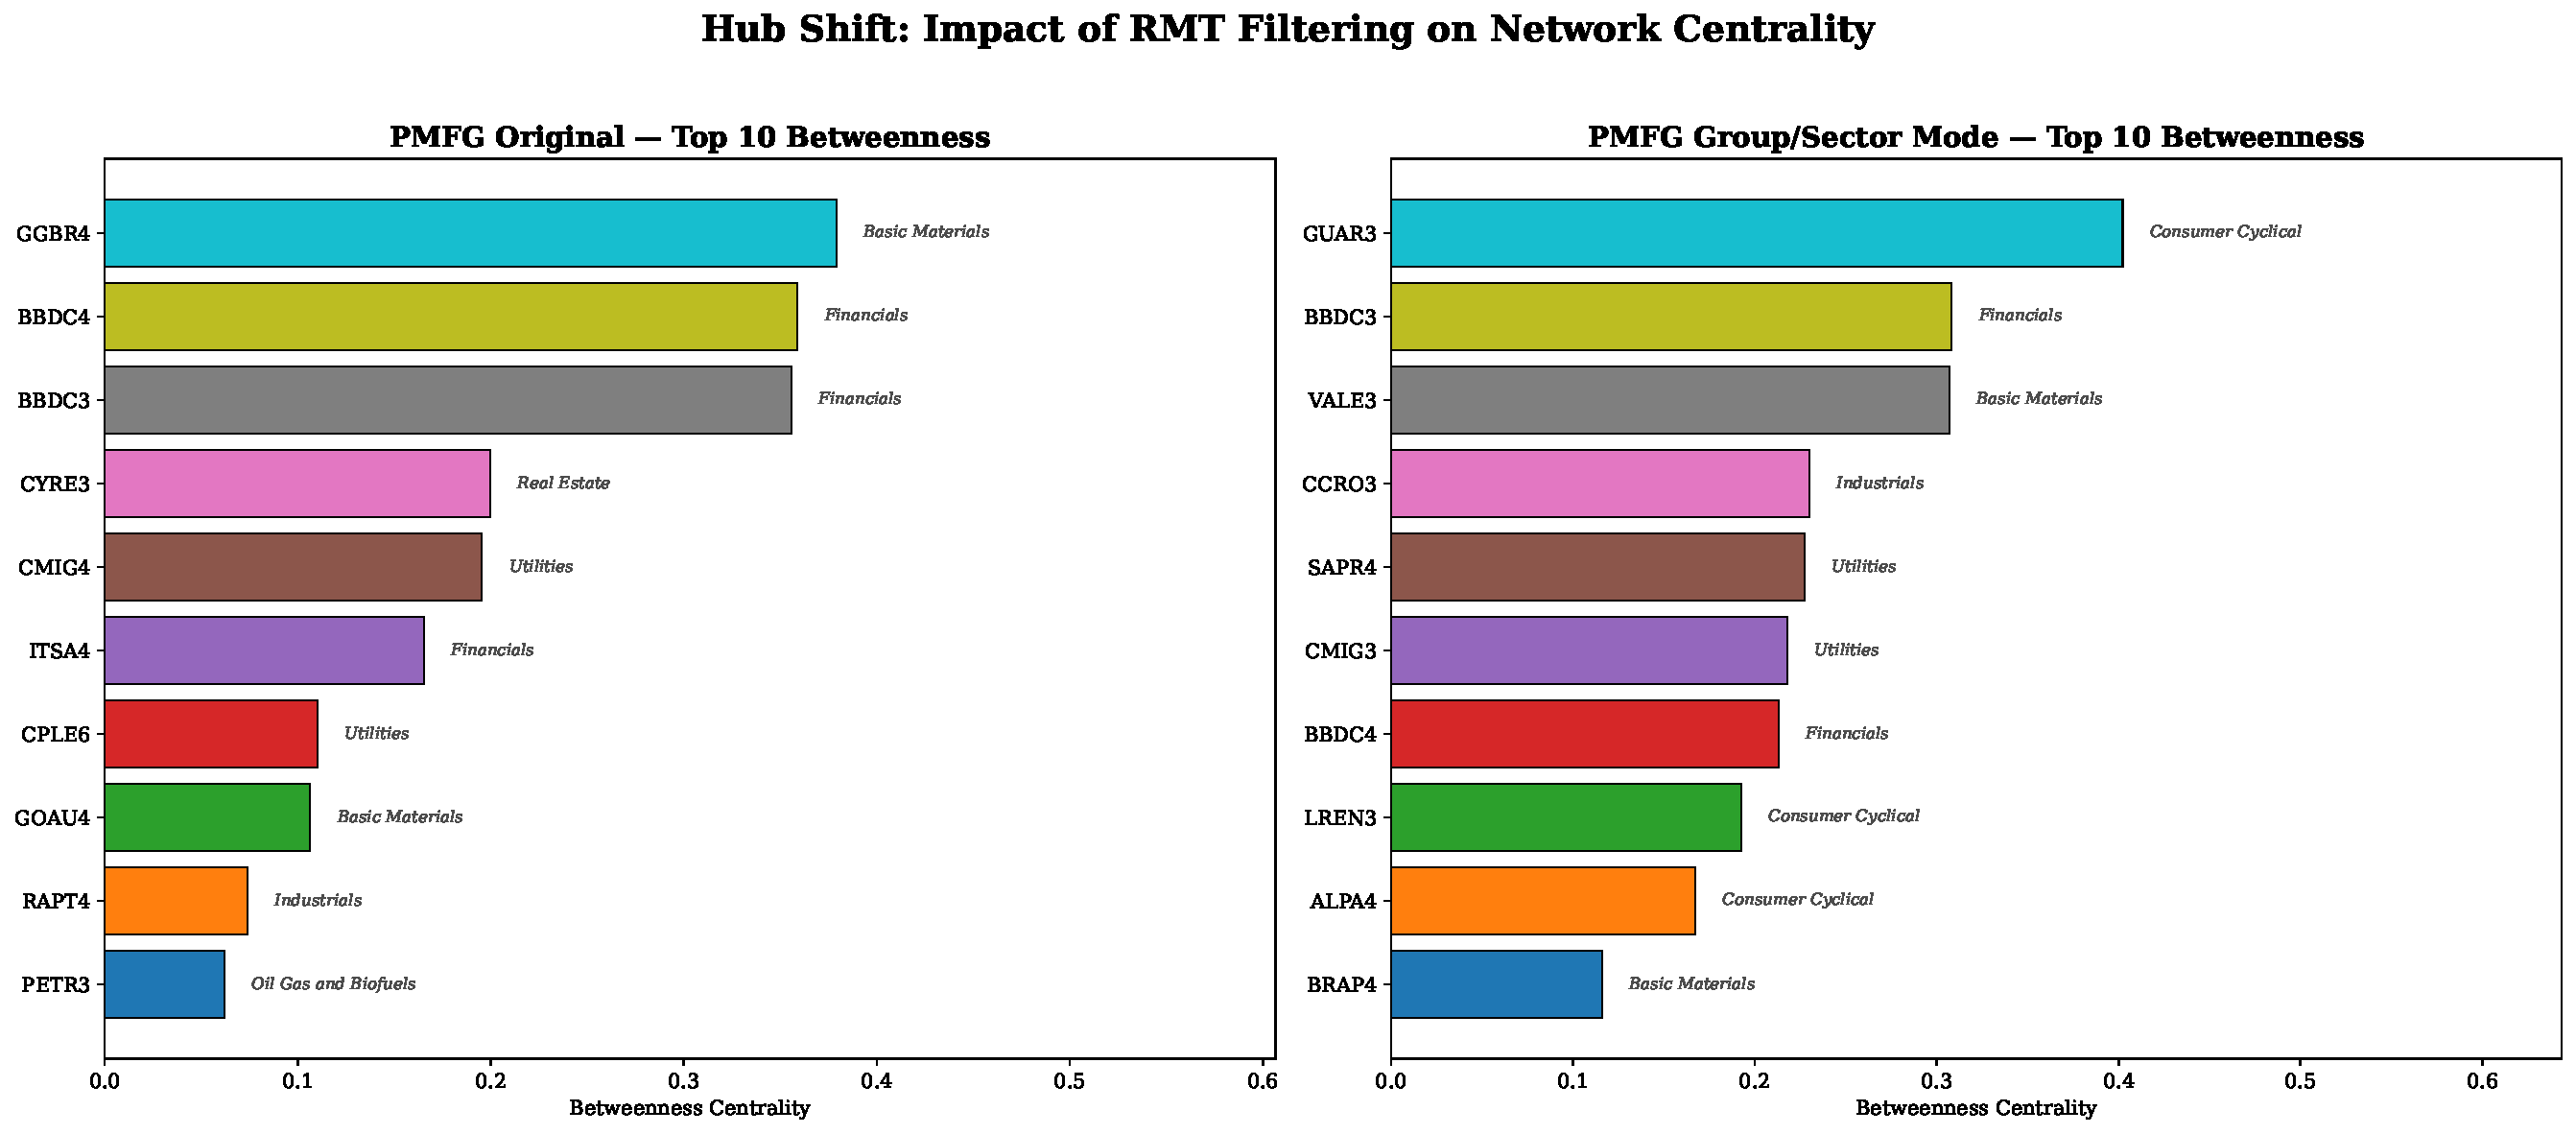
\includegraphics[
width=\linewidth,
height=0.58\textheight,
keepaspectratio
]{images/figure_14_network_hub_rank_comparison.pdf}
\captionof{figure}{Hub-rank comparison across original and group-mode networks. Removal of the dominant market component changes which assets occupy central positions in the dependency structure.}
\label{fig:hub_rank}
\end{center}



\begin{center}
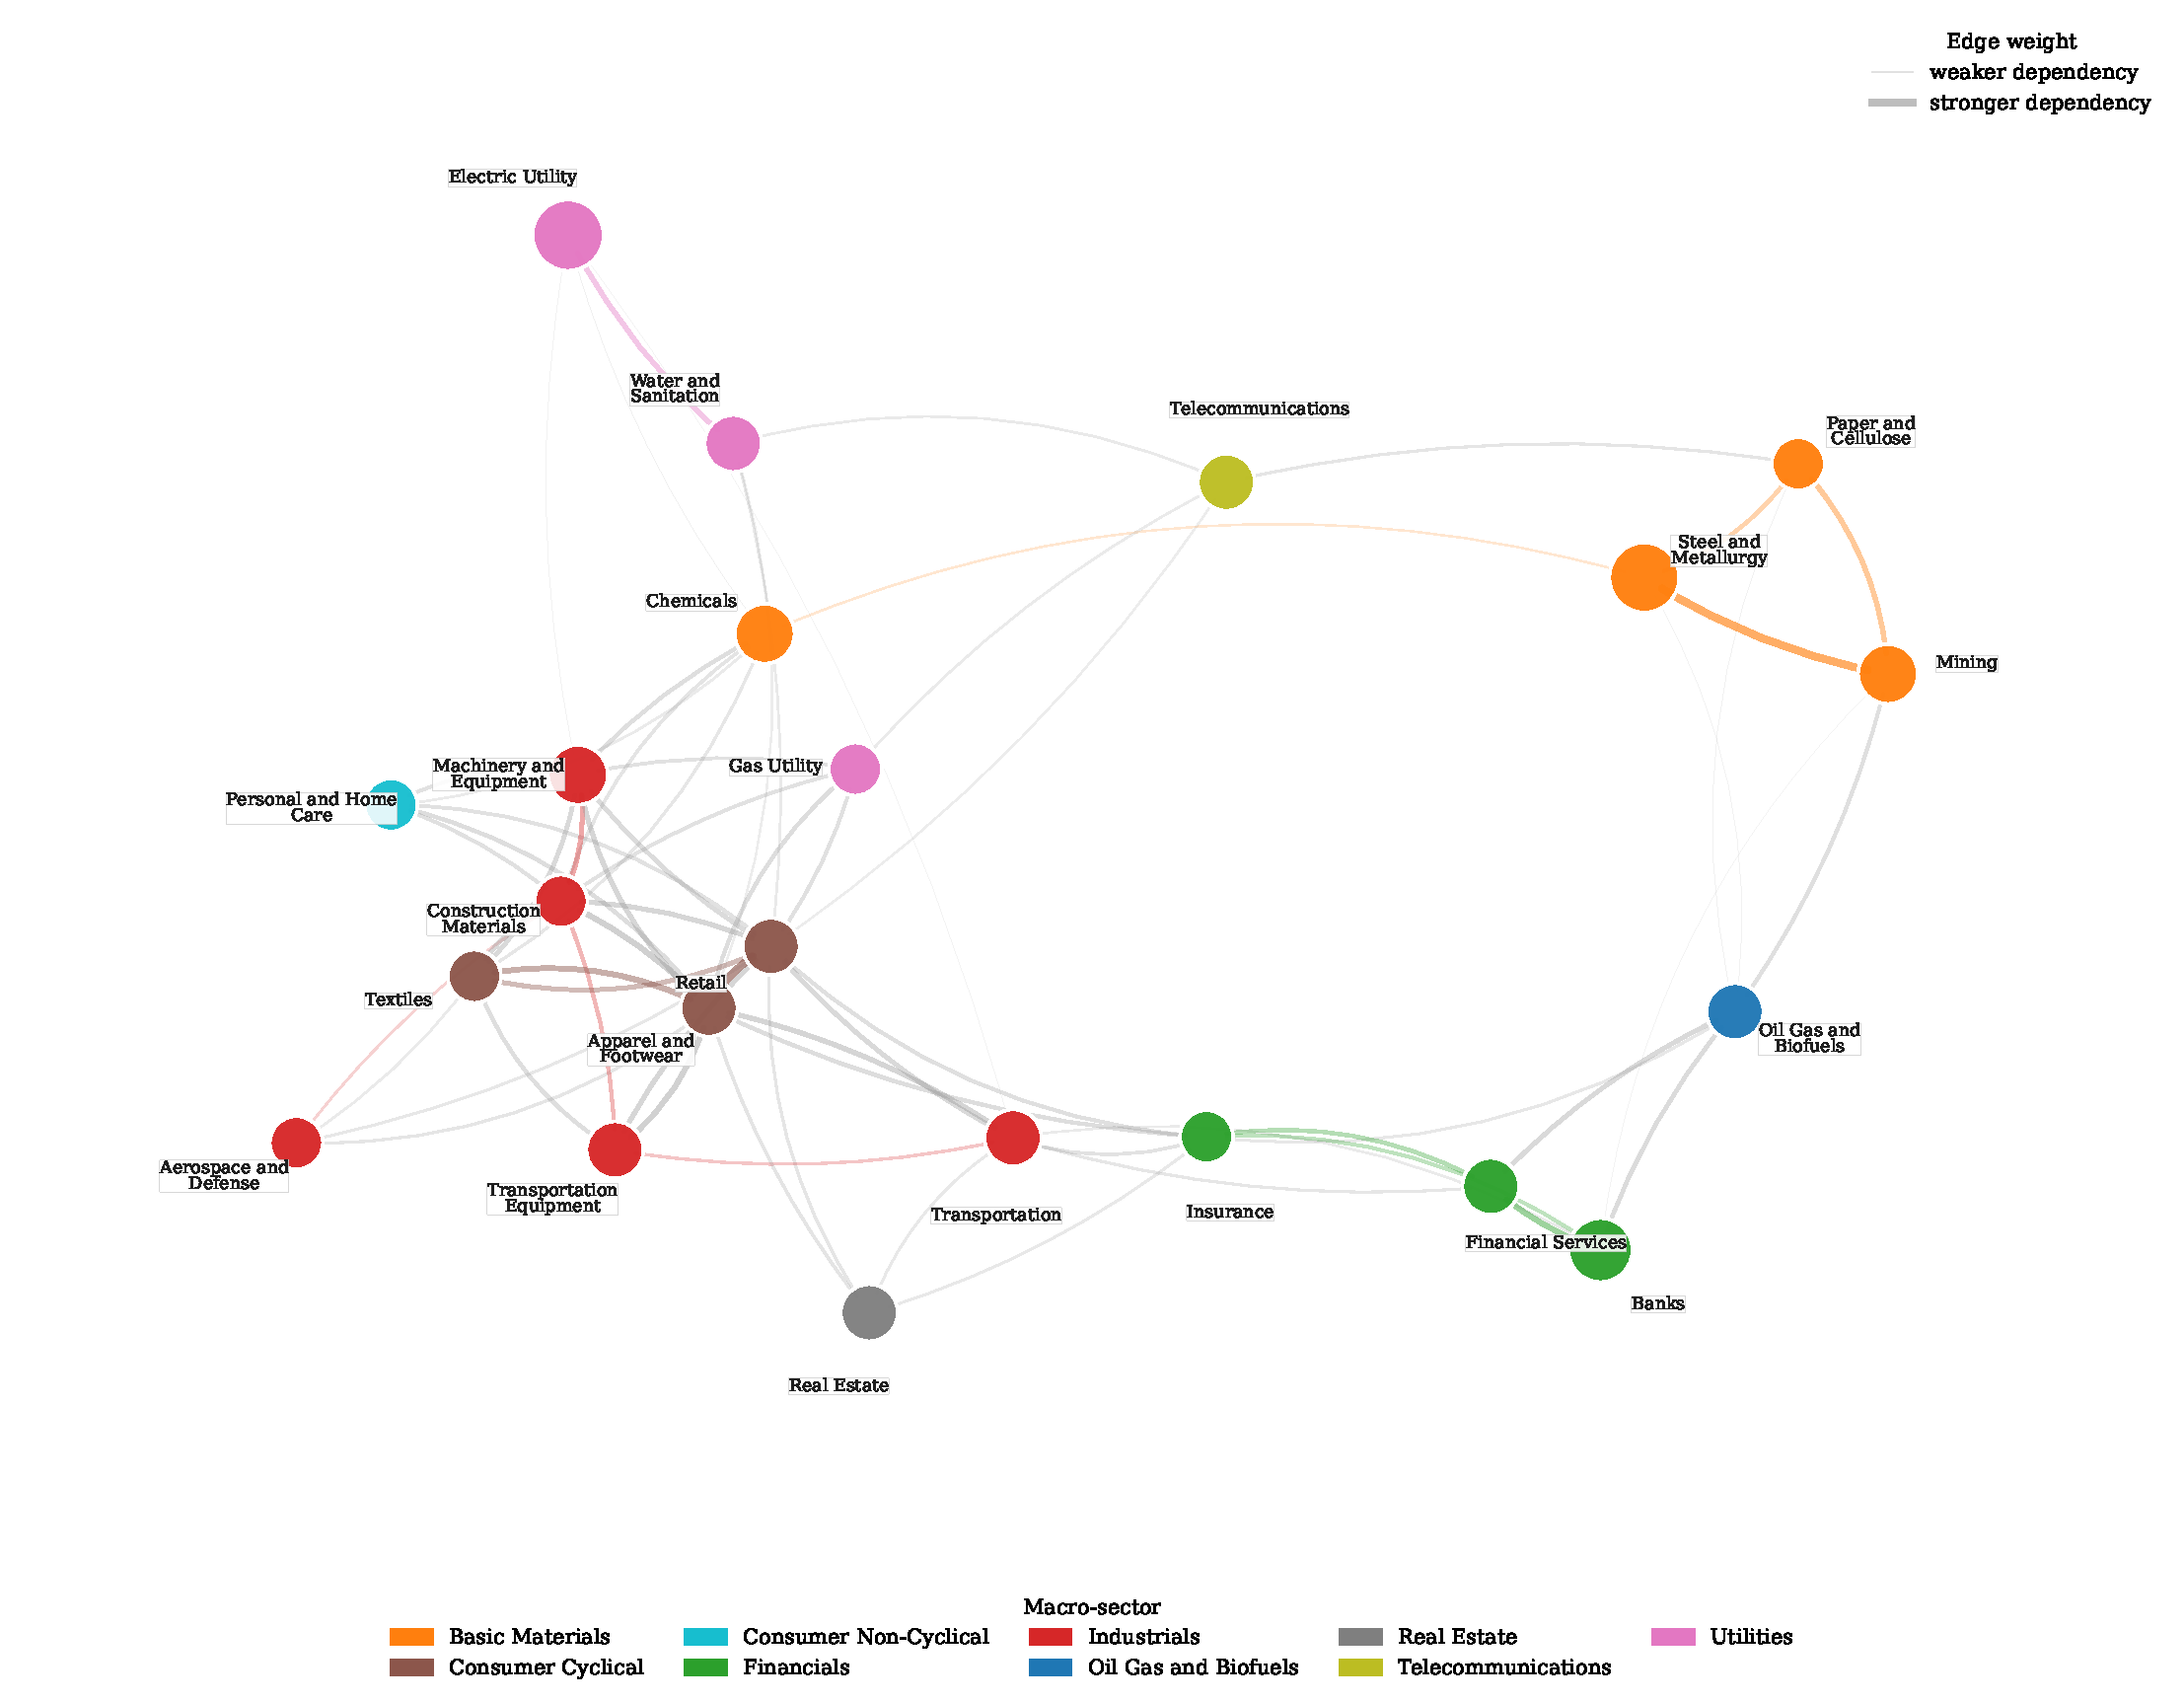
\includegraphics[
width=0.92\linewidth,
height=0.58\textheight,
keepaspectratio
]{images/figure_15_subsector_dependency_network.pdf}
\captionof{figure}{Aggregated subsector dependency network. Nodes represent subsectors, node colour identifies the macro-sector and node size is proportional to the number of assets in each subsector. Edge thickness represents the average retained dependency between connected subsectors.}
\label{fig:subsector_network}
\end{center}

The original-network hubs can reflect both localized relationships and exposure to the broad common component. After market-mode removal, the central nodes instead characterize the residual dependency structure. Assets such as GUAR3, BBDC3, VALE3, CCRO3, SAPR4 and CMIG3 consequently gain prominence in the group-mode rankings. These rankings are interpreted as descriptive full-sample configurations rather than permanent structural labels, since their temporal stability is examined separately in Section~\ref{sec:robustness}.

To translate this ticker-level organization into a more interpretable economic representation, we aggregate the retained dependencies by subsector. The resulting network contains 22 subsectors and 66 undirected links, with density 0.2857. Its mean and median edge dependencies are 0.0566 and 0.0561, respectively. These relatively small values are expected because the graph summarizes dependencies after spectral filtering and aggregation rather than raw pairwise correlations.

Figure~\ref{fig:subsector_network} shows the resulting subsector-level structure. Nodes represent subsectors, node colours indicate macro-sectors, and node sizes reflect the number of constituent assets. Edge thickness represents the average retained dependency between the corresponding subsectors.

The aggregated network reveals different forms of structural importance. Retail has the highest degree, indicating the largest number of retained direct subsector connections. Electric Utility has the highest betweenness, placing it in a bridge-like position between different parts of the graph. Apparel and Footwear has the highest weighted degree, indicating that its retained connections are comparatively strong. These differences show that connectivity, bridging position, and dependency intensity capture distinct aspects of the residual market structure.

The subsector representation therefore provides an economic summary of the organization identified previously at the spectral and ticker-network levels. The analysis begins with non-leading RMT modes, shows that localized structure persists in hierarchical and graph representations, and finally translates the retained network relationships into sectoral and subsector-level organization. This completes the structural part of the empirical analysis before the robustness tests and retrospective volatility-model assessment.


\subsection{Robustness of the Structural Findings}
\label{sec:robustness}

The preceding results identify sectoral organization, significant non-leading spectral modes, and a reorganization of hierarchical and network structure after removal of the dominant market component. We now examine whether these findings remain when key features of the analysis are challenged. The robustness analysis focuses on three potential sensitivities: the economic labels assigned to assets, the presence of multiple share classes from the same issuer, and the stability of the resulting network structure across time.

\subsubsection{Robustness of the Sectoral and Spectral Structure}

The sectoral pattern identified in Section~\ref{sec:stylized_correlation} is tested using an asset-level label-permutation procedure that preserves both the empirical dependency matrix and the observed sector-size distribution. The observed difference between mean within-sector and between-sector correlations is $\Delta_{\mathrm{sector}}=0.1184$, whereas the 95th percentile of the permutation distribution is 0.0245. None of the 10,000 permutations produces a difference as large as the observed value ($p\approx 10^{-4}$, the minimum attainable at this simulation count). The stronger within-sector dependence is therefore not reproduced by random reassignment of the existing sector labels.

A separate robustness concern arises from companies represented by multiple listed share classes. The 58-asset panel contains 12 such issuers, which can strengthen issuer-specific co-movement and generate localized spectral components. We therefore repeat the RMT analysis after retaining one deterministic representative per company, reducing the cross-section to 46 issuers.

\begin{center}
\captionof{table}{Issuer-level RMT robustness check on the same 1,527 dates as the full panel. Parentheses give the number of non-market modes above the Mar\v{c}enko--Pastur upper bound.}
\label{tab:issuer_rmt_robustness}
\small
\resizebox{\linewidth}{!}{%
\begin{tabular}{lrrrrrrr}
\toprule
Panel & $N$ & $T$ & $Q$ & $\lambda_{+}$ & Eigenvalues above $\lambda_{+}$ & $\lambda_{1}/N$ & Mean pairwise corr. \\
\midrule
Full share-class panel & 58 & 1527 & 26.33 & 1.4278 & 5 (4) & 0.3733 & 0.3350 \\
Issuer-collapsed panel & 46 & 1527 & 33.20 & 1.3773 & 3 (2) & 0.3611 & 0.3215 \\
\bottomrule
\end{tabular}}
\end{center}



Both panels use the common dates 23 August 2006--15 August 2024, so this comparison changes the cross-section while holding the observation period fixed. Issuer representatives are selected by common-panel coverage, then mean financial volume over those same dates, then ticker as a deterministic final tie-break. The rule retains PETR4 over PETR3, ELET3 over ELET6, and CPLE6 over CPLE3. The leading trace share is 0.3733 in the full panel and 0.3611 after collapse. Four non-market eigenvalues exceed the full-panel bound, compared with two in the issuer panel (2.2912 and 1.5388). Thus the number of candidate group modes is sensitive to share-class representation even when $T$ is held constant.

The group-mode matrix and both graph families were recomputed for the two panels on these same dates. Table~\ref{tab:issuer_network_robustness} reports the group-mode network summaries; it separates the effect of reducing $N$ from the prior comparison, which also changed $T$.

\begin{center}
\captionof{table}{MST and PMFG summaries for the group-mode matrices recomputed on the same dates.}
\label{tab:issuer_network_robustness}
\small
\resizebox{\linewidth}{!}{%
\begin{tabular}{llrrrrrr}
\toprule
Panel & Network & Assets & Edges & Mean edge corr. & Same-sector ratio & Clustering & Top degree / betweenness \\
\midrule
Full share-class & MST & 58 & 57 & 0.1388 & 0.6316 & 0.0000 & ALPA4 / ALPA4 \\
Issuer-collapsed & MST & 46 & 45 & 0.0982 & 0.6000 & 0.0000 & CMIG4 / SHUL4 \\
Full share-class & PMFG & 58 & 168 & 0.1109 & 0.5417 & 0.6653 & GUAR3 / GUAR3 \\
Issuer-collapsed & PMFG & 46 & 132 & 0.0812 & 0.4621 & 0.6761 & ROMI3 / SAPR4 \\
\bottomrule
\end{tabular}}
\end{center}



After issuer collapse, mean group-mode edge correlation decreases for both the MST and PMFG, while PMFG average clustering is similar. The edge counts equal $N-1$ and $3N-6$, respectively, in each panel. These changes describe sensitivity to cross-sectional composition; the analysis does not attribute them to a change in sample dates.

We further test the spectral results against a circular-shift surrogate null. Each surrogate preserves the marginal distribution and temporal ordering of every individual return series while breaking their contemporaneous alignment across assets. Across 1,000 independent surrogate realizations, empirical ranks 1--5 exceed their rank-matched 95th-percentile thresholds. Rank 6 is the first that does not: its empirical value is 1.1673, below the null 95th percentile of 1.3057; ranks 6--58 have 1,000 of 1,000 surrogate values at least as large as the empirical value ($p=1$ under the plus-one estimate). For ranks 1--5, zero exceedances give $p=1/(1,001)\approx0.001$, the minimum attainable. This identifies where the empirical spectrum ceases to exceed the circular-shift null.

The issuer-collapse and circular-shift results should be interpreted jointly. The surrogate experiment supports the presence of genuine cross-sectional synchronization beyond the null benchmark, whereas the issuer-level experiment shows that the economic interpretation of some weaker modes remains sensitive to the representation of multiple share classes. Robust statistical separation from the null therefore does not imply that every significant mode corresponds to a broad or stable economic factor.

\subsubsection{Temporal Stability of the Network Structure}

The full-sample MST and PMFG representations summarize long-run dependency structure, but their individual edges and central nodes need not remain unchanged through time. To examine this sensitivity, the synchronized sample is divided into three consecutive windows of 509 observations and the networks are re-estimated within each window. Table~\ref{tab:network_temporal_stability} summarizes the mean pairwise overlap across the resulting network realizations.

\begin{center}
\captionof{table}{Temporal stability of the MST and PMFG structures across three consecutive windows. Values are means across window pairs.}
\label{tab:network_temporal_stability}

\small
\begin{tabular}{llrrr}
\toprule
Network & Matrix & Edge Jaccard & Top-5 hub overlap & Community ARI \\
\midrule
MST & Original & 0.206 & 0.267 & 0.138 \\
MST & Group mode & 0.047 & 0.200 & 0.182 \\
PMFG & Original & 0.212 & 0.200 & 0.214 \\
PMFG & Group mode & 0.140 & 0.200 & 0.174 \\
\bottomrule
\end{tabular}
\end{center}



Edge persistence is modest in the original networks and lower still for several group-mode comparisons. The mean edge Jaccard similarity is 0.206 for the original MST and 0.212 for the original PMFG, compared with 0.047 and 0.140 for their group-mode counterparts. Hub persistence is also limited: mean overlap among the five highest-betweenness nodes ranges from 0.20 to 0.27, and no top-five betweenness hub appears in all three windows. Community agreement, measured by the adjusted Rand index, is similarly modest.

These results qualify the interpretation of the full-sample networks. The structural analyses in Section~\ref{sec:network_organization} identify meaningful long-run dependency configurations, but individual edges, hub identities, and community assignments should not be interpreted as invariant properties of the Brazilian equity market. This distinction is particularly important for the retrospective volatility assessment that follows, where full-sample structural descriptors are used as ex-post characteristics rather than as point-in-time network estimates.


\subsection{Retrospective Volatility-Model Assessment}
\label{sec:forecasting}

The preceding analyses identify cross-sectional dependency structure in B3 equities. We now ask whether adding structural descriptors improves realized-volatility forecast accuracy. The RMT and network descriptors are estimated from the full synchronized sample, so this is a retrospective comparison rather than a point-in-time forecasting design.

The chronological test period is 2021--2025. Specifications are selected by mean validation QLIKE within each model family and feature set; no test-period metric is used for selection. Figure~\ref{fig:forecast_comparison} shows aggregated test QLIKE. Lower values indicate lower loss. The confidence intervals are circular moving-block bootstrap intervals and are descriptive; paired HAC tests provide the focused feature-set comparisons below.

\begin{center}
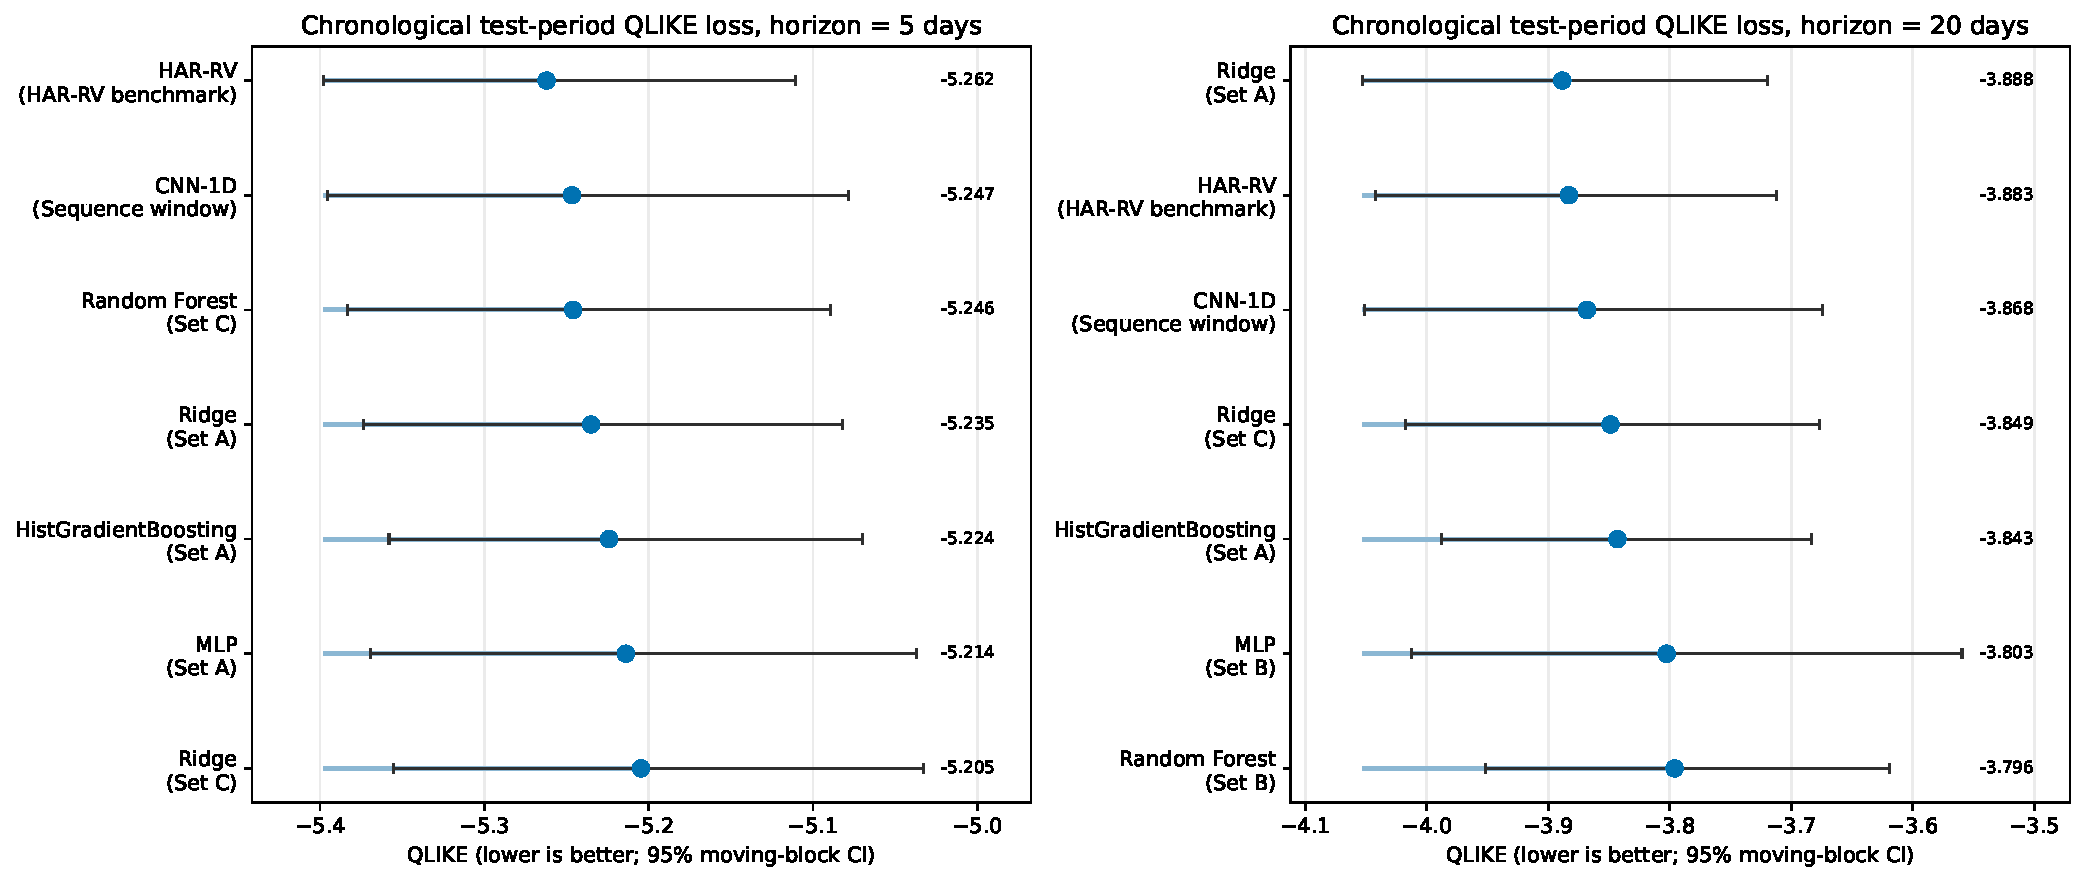
\includegraphics[width=\linewidth,height=0.58\textheight,keepaspectratio]{images/figure_16_volatility_forecast_model_comparison.pdf}
\captionof{figure}{Chronological test-period QLIKE across validation-selected specifications. Points show the mean across PETR4, VALE3 and BBDC4; bars show 95\% circular moving-block bootstrap intervals from 2,000 replications, with block length equal to the forecast horizon.}
\label{fig:forecast_comparison}
\end{center}

HAR-RV has the lowest mean QLIKE at the 5-day horizon; at 20 days, the explicit Ridge Set A comparator has a slightly lower mean than HAR-RV. The bootstrap intervals overlap substantially, so these descriptive rankings do not establish that either specification is significantly better than every alternative. The primary structural comparison is between validation-selected Ridge Set A and Ridge Set B/C, because these specifications isolate the addition of market/RMT and network descriptors while keeping the model family fixed.

Table~\ref{tab:forecast_comparison} gives validation-selected test summaries, the explicit Ridge Set A comparator, and HAR-RV. The asset-level results, block-length sensitivity and five-seed neural sensitivity are reported in Tables~\ref{tab:app_forecast},~\ref{tab:app_blocks} and~\ref{tab:app_seeds}.

\begin{center}
\captionof{table}{Validation-selected model results and the fixed Ridge Set A comparator on the 2021--2025 test period. Metrics are averaged across PETR4, VALE3 and BBDC4.}
\label{tab:forecast_comparison}
\resizebox{\linewidth}{!}{%
\begin{tabular}{lllrrrrr}
\toprule
Horizon & Model & Feature set & MAE & RMSE & QLIKE & 95\% CI for QLIKE & $R^2_{\mathrm{oos}}$ \\
\midrule
5 & CNN-1D & Sequence window & 0.0145 & 0.0213 & $-5.2467$ & $[-5.3955, -5.0784]$ & 0.2871 \\
5 & Random Forest & Set C (+Network) & 0.0162 & 0.0227 & $-5.2460$ & $[-5.3834, -5.0895]$ & 0.2001 \\
5 & HistGradientBoosting & Set A (Classical) & 0.0168 & 0.0235 & $-5.2241$ & $[-5.3581, -5.0700]$ & 0.1468 \\
5 & MLP & Set A (Classical) & 0.0138 & 0.0209 & $-5.2139$ & $[-5.3692, -5.0369]$ & 0.3150 \\
5 & Ridge & Set C (+Network) & 0.0146 & 0.0215 & $-5.2047$ & $[-5.3553, -5.0329]$ & 0.2733 \\
20 & CNN-1D & Sequence window & 0.0210 & 0.0308 & $-3.8682$ & $[-4.0509, -3.6740]$ & 0.3947 \\
20 & Ridge & Set C (+Network) & 0.0224 & 0.0316 & $-3.8487$ & $[-4.0177, -3.6765]$ & 0.3587 \\
20 & HistGradientBoosting & Set A (Classical) & 0.0265 & 0.0375 & $-3.8430$ & $[-3.9879, -3.6834]$ & 0.1560 \\
20 & MLP & Set B (+Market/RMT) & 0.0220 & 0.0322 & $-3.8026$ & $[-4.0126, -3.5595]$ & 0.3514 \\
20 & Random Forest & Set B (+Market/RMT) & 0.0284 & 0.0405 & $-3.7960$ & $[-3.9514, -3.6195]$ & 0.0124 \\
5 & Ridge (Set A baseline) & Set A (Classical) & 0.0146 & 0.0213 & $-5.2351$ & $[-5.3736, -5.0820]$ & 0.2813 \\
5 & HAR-RV & HAR-RV benchmark & 0.0157 & 0.0222 & $-5.2622$ & $[-5.3978, -5.1109]$ & 0.2228 \\
20 & Ridge (Set A baseline) & Set A (Classical) & 0.0217 & 0.0306 & $-3.8884$ & $[-4.0528, -3.7198]$ & 0.3941 \\
20 & HAR-RV & HAR-RV benchmark & 0.0240 & 0.0335 & $-3.8830$ & $[-4.0422, -3.7123]$ & 0.2826 \\
\bottomrule
\end{tabular}}
\end{center}

\noindent\footnotesize\emph{Notes:} QLIKE is defined in Eq.~\eqref{eq:theory_qlike}; $R^2_{\mathrm{oos}}$ is relative to the training-sample mean benchmark. Set A contains point-in-time return and volatility predictors; Set B adds market and full-sample RMT descriptors; Set C additionally includes full-sample MST and PMFG descriptors. Sets B and C are retrospective structural specifications.
\normalsize

We compare validation-selected Ridge Set B/C with Ridge Set A using date-level mean QLIKE differences across the three assets and Newey--West standard errors with horizon-specific lags. The same test also reports HAR-RV versus Ridge Set A. The difference is defined as baseline QLIKE minus candidate QLIKE, so a positive value favours the candidate. Table~\ref{tab:forecast_loss_test} reports two-sided $p$-values; Holm adjustment is applied across the four structural contrasts.

\begin{center}
\captionof{table}{HAC tests of validation-selected feature-set contrasts and HAR-RV against Ridge Set A. Negative differences favour the Set A baseline.}
\label{tab:forecast_loss_test}
\resizebox{\linewidth}{!}{%
\begin{tabular}{rlrrrrrr}
\toprule
Horizon & Contrast & Mean difference & HAC s.e. & Statistic & Two-sided $p$ & Holm $p$ \\
\midrule
5 & Set B vs Set A & -0.023021 & 0.006010 & -3.831 & 0.000128 & 0.000384 \\
5 & Set C vs Set A & -0.030401 & 0.007332 & -4.147 & 0.000034 & 0.000135 \\
20 & Set B vs Set A & -0.029578 & 0.010914 & -2.710 & 0.006727 & 0.006727 \\
20 & Set C vs Set A & -0.039761 & 0.011464 & -3.468 & 0.000524 & 0.001047 \\
5 & HAR-RV vs Ridge A & -0.027097 & 0.015080 & -1.797 & 0.072348 & -- \\
20 & HAR-RV vs Ridge A & 0.005454 & 0.011444 & 0.477 & 0.633657 & -- \\
\bottomrule
\end{tabular}}
\end{center}

\noindent\footnotesize\emph{Notes:} The loss difference is QLIKE$_{\mathrm{Ridge\ A}}-$QLIKE$_{\mathrm{candidate}}$, averaged by date across the three assets. Newey--West lags are 4 and 19 for the 5- and 20-day horizons. Holm adjustment covers the four Set B/C versus Set A tests; HAR-RV contrasts are shown separately and are not included in that family.
\normalsize

All four Ridge Set B/C contrasts have negative mean differences, and their two-sided HAC tests remain significant after Holm adjustment. Thus, in this retrospective test, adding the structural feature sets does not improve QLIKE over Ridge Set A; the observed losses are higher. The HAR-RV versus Ridge Set A comparison is not significant at either horizon. These results answer the accuracy question for the evaluated pooled assets and split, but do not establish performance for recursively estimated, point-in-time structural features.

\begin{center}
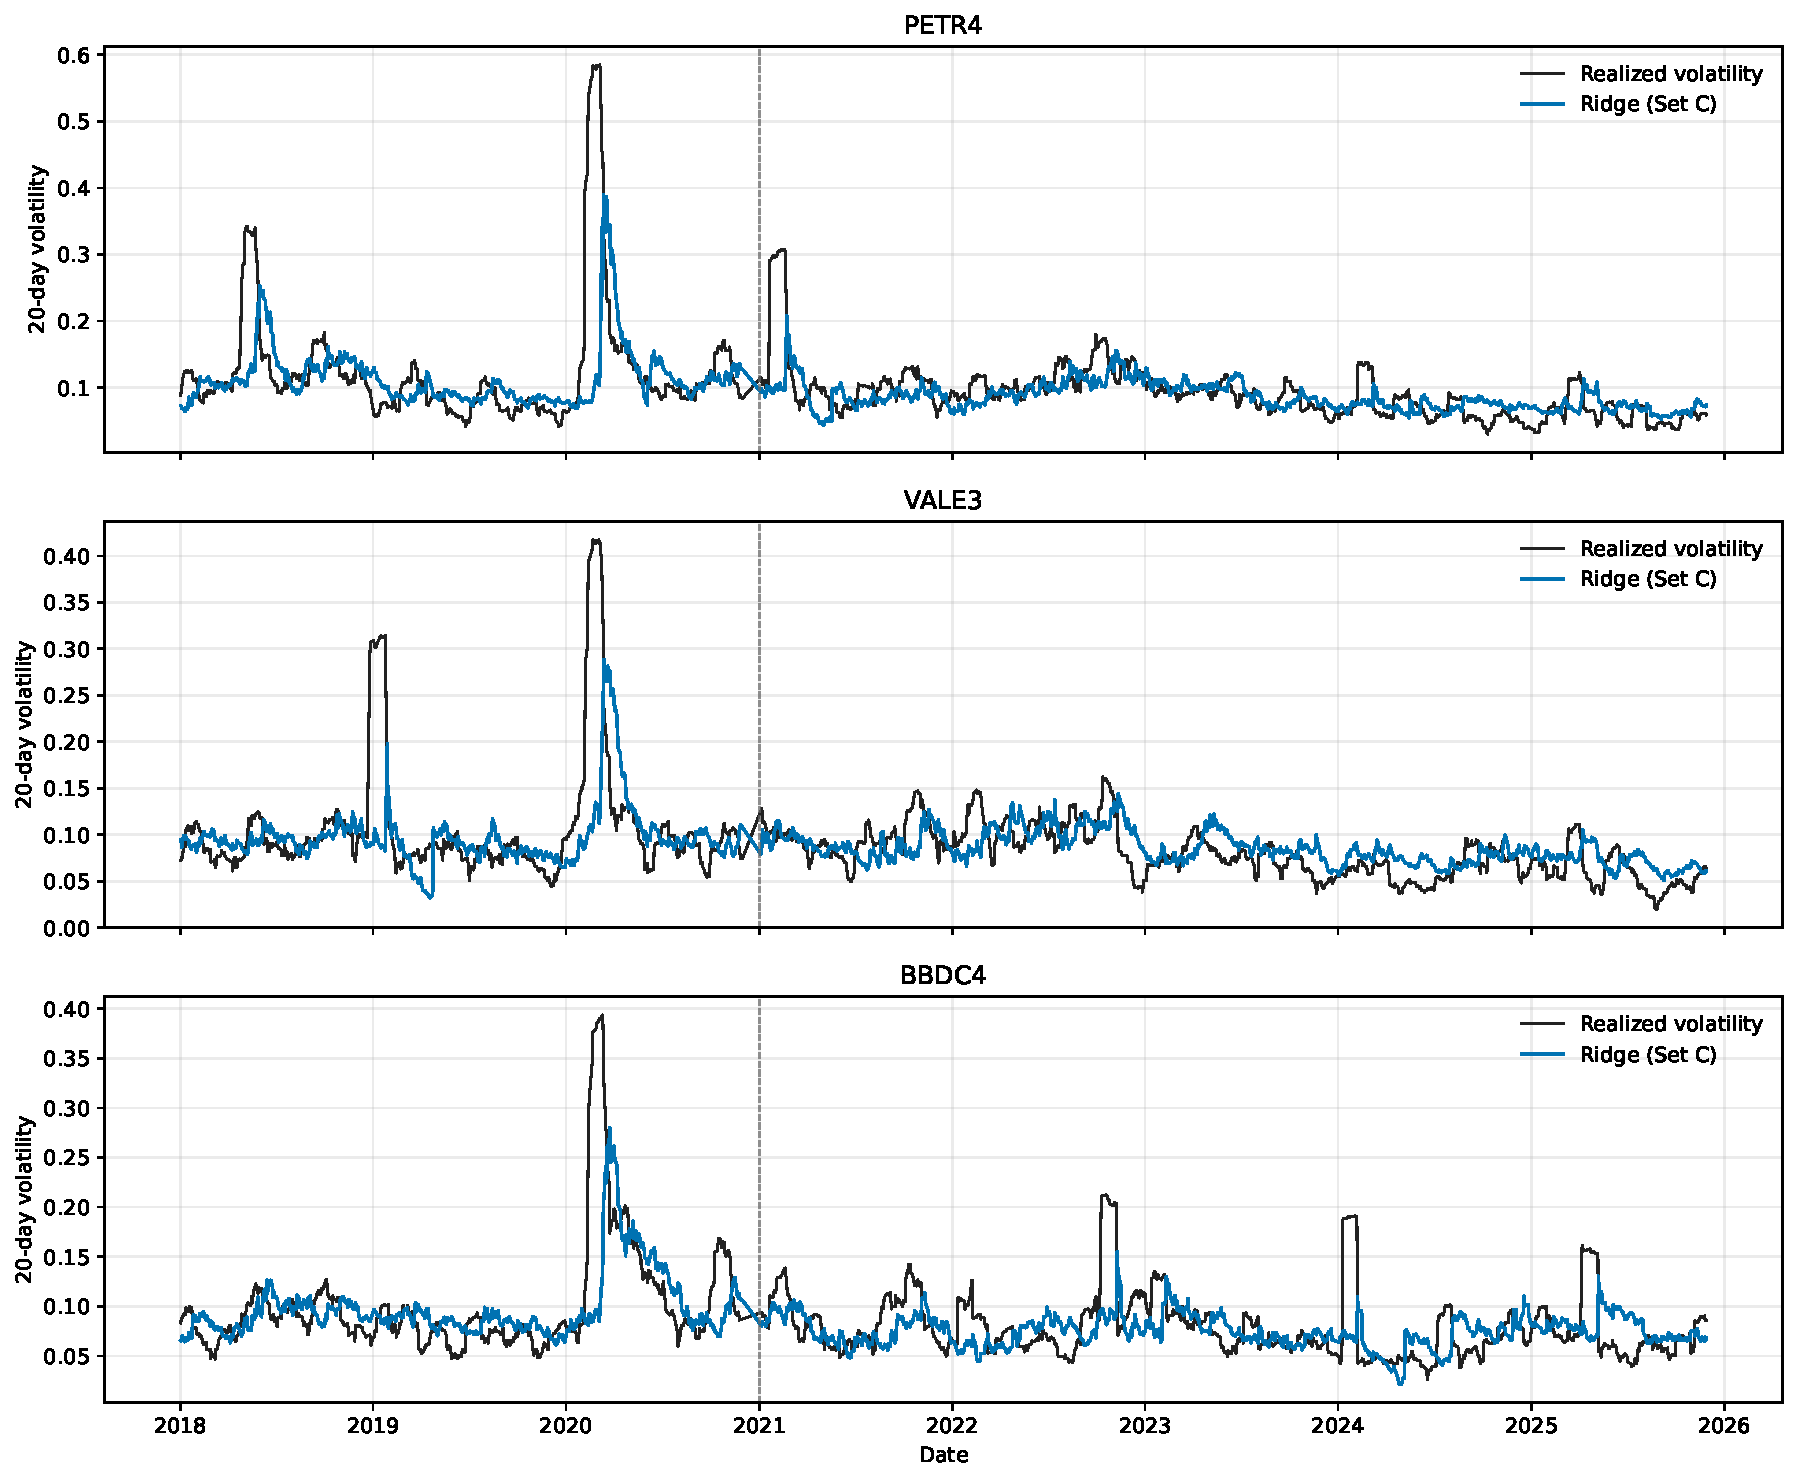
\includegraphics[width=0.95\linewidth,height=0.58\textheight,keepaspectratio]{images/figure_17_realized_vs_predicted_volatility.pdf}
\captionof{figure}{Realized and predicted 20-day volatility for PETR4, VALE3 and BBDC4 using the specification selected on validation data. The vertical dashed line marks the beginning of the 2021--2025 test period.}
\label{fig:realized_vs_predicted}
\end{center}

Figure~\ref{fig:realized_vs_predicted} shows that forecasts follow persistent volatility changes but smooth abrupt realized spikes and subsequent reversals. This visual pattern complements, but does not replace, the aggregate loss comparisons.

Figure~\ref{fig:feature_importance} reports the largest Random Forest impurity-based importance entries across candidate feature sets at each horizon. These values describe how fitted trees use predictors; they do not estimate marginal forecast gains or causal contributions.

\begin{center}
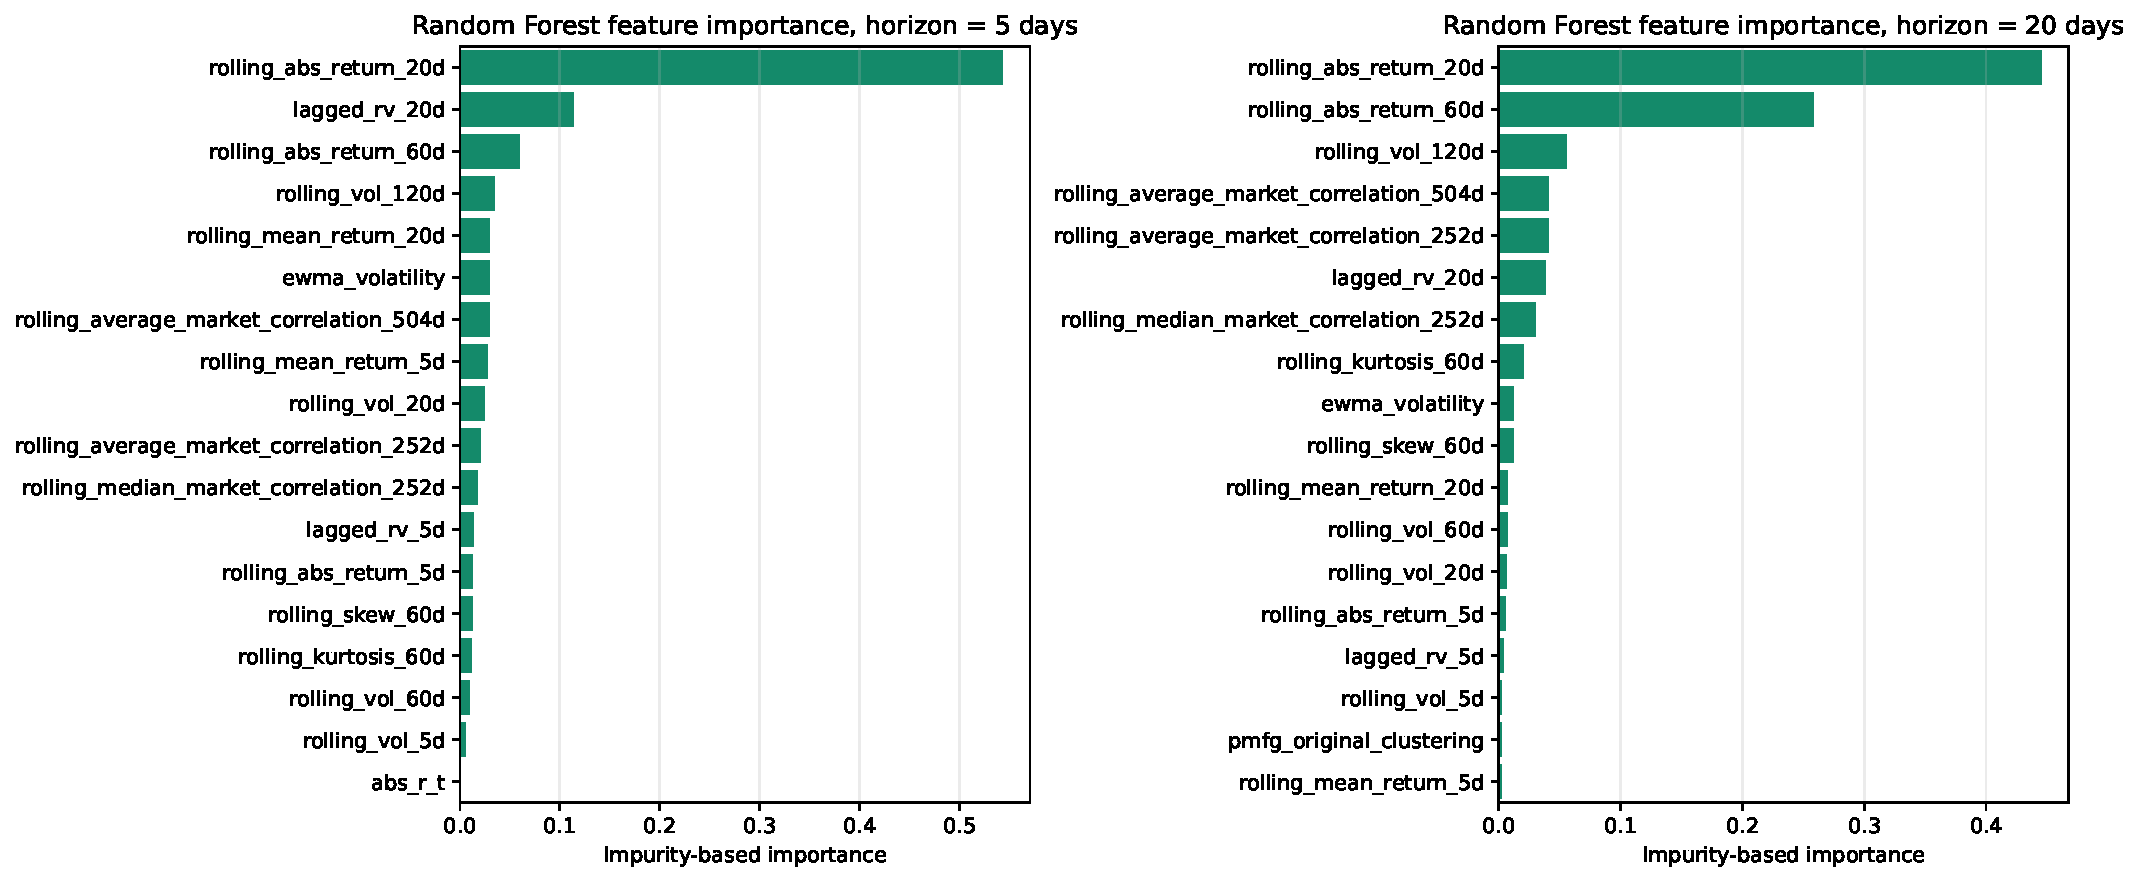
\includegraphics[width=0.95\linewidth,height=0.58\textheight,keepaspectratio]{images/figure_18_ml_feature_importance.pdf}
\captionof{figure}{Random Forest impurity-based importance for the validation-selected feature set at each horizon. Importance is descriptive and is not a measure of incremental predictive value.}
\label{fig:feature_importance}
\end{center}

Conventional volatility predictors account for most of the highest-ranked entries. Structural descriptors also appear in selected models, but their presence among tree splits does not override the test result: the paired Ridge comparisons do not show an accuracy gain from Set B or Set C. Neural-seed sensitivity and block-length sensitivity are documented in Tables~\ref{tab:app_seeds} and~\ref{tab:app_blocks}.

